\documentclass[11pt,a4paper]{article}

\usepackage[top=1in,bottom=1in,left=1in,right=1in]{geometry}
\usepackage[utf8]{inputenc}
\usepackage[T1]{fontenc}
\usepackage{amsmath,amssymb,amsfonts,amsthm}
\usepackage{lmodern}
\usepackage{microtype}
\usepackage{graphicx}
\usepackage{booktabs}
\usepackage{multirow}
\usepackage{tabularx}
\usepackage{xcolor}
\usepackage{listings}
\usepackage{algorithm}
\usepackage{algpseudocode}
\usepackage{hyperref}
\usepackage{cite}
\usepackage{subcaption}
\usepackage{titlesec}
\usepackage{fancyhdr}
\usepackage{setspace}

\setstretch{1.15}

% Clean section title styling
\titleformat{\section}{\large\bfseries\color{blue!75!black}}{\thesection}{1em}{}[\vspace{0.4ex}\titlerule]
\titleformat{\subsection}{\normalsize\bfseries\color{black!90}}{\thesubsection}{1em}{}
\titleformat{\subsubsection}{\small\bfseries\color{black!75}}{\thesubsubsection}{1em}{}

% Running headers and footers (arXiv style)
\pagestyle{fancy}
\fancyhf{}
\lhead{\footnotesize \textit{arXiv Preprint --- Quantitative Biology / Machine Learning}}
\rhead{\footnotesize \textit{Srivastava (IIT Kanpur)}}
\cfoot{\thepage}
\renewcommand{\headrulewidth}{0.4pt}
\setlength{\headheight}{14pt}

% Hyperlink configuration
\hypersetup{
    colorlinks=true,
    linkcolor=blue!70!black,
    citecolor=green!50!black,
    urlcolor=blue!80!black
}

% Code listing styling with properly padded left margins
\definecolor{codegreen}{rgb}{0,0.55,0.2}
\definecolor{codegray}{rgb}{0.45,0.45,0.45}
\definecolor{codepurple}{rgb}{0.55,0,0.75}
\definecolor{codeblue}{rgb}{0.1,0.25,0.75}
\definecolor{backcolour}{rgb}{0.975,0.98,0.99}

\lstdefinestyle{pythonstyle}{
    backgroundcolor=\color{backcolour},   
    commentstyle=\color{codegreen}\itshape,
    keywordstyle=\color{codeblue}\bfseries,
    numberstyle=\tiny\color{codegray},
    stringstyle=\color{codepurple},
    basicstyle=\ttfamily\footnotesize,
    breakatwhitespace=false,         
    breaklines=true,                 
    captionpos=b,                    
    keepspaces=true,                 
    numbers=left,                    
    numbersep=10pt,                  
    xleftmargin=2.5em,
    frame=single,
    framexleftmargin=2.0em,
    rulecolor=\color{black!15},
    showspaces=false,                
    showstringspaces=false,
    showtabs=false,                  
    tabsize=4
}
\lstset{style=pythonstyle}

\begin{document}

% =========================================================================
% TITLE AND METADATA BLOCK
% =========================================================================
\begin{center}
    {\Large \bfseries Graph Neural Networks and Gradient-Boosted Tree Hybrid Stacking for Coarse-Grained Molecular Force Field Parameterization} \\[2.0ex]
    
    \textbf{Shaurya Srivastava} \\[0.8ex]
    \textit{Department of Electrical Engineering, Indian Institute of Technology Kanpur (IIT Kanpur)} \\
    \textit{Kanpur, Uttar Pradesh 208016, India} \\
    \texttt{shauryas21@iitk.ac.in} \\[1.5ex]
    
    \textbf{Open-Source Code \& Checkpoints:} \url{https://github.com/shaurya244/EE798-CG-ForceField-GNN} \\[1.5ex]
    \rule{\textwidth}{0.8pt}
\end{center}

\vspace{-0.5em}

% =========================================================================
% ABSTRACT
% =========================================================================
\begin{abstract}
\noindent Determining bonded interaction parameters ($k_{\text{bond}}, r_0, k_{\text{angle}}, \theta_0$) for coarse-grained (CG) molecular force fields---predominantly MARTINI~3---conventionally requires weeks of computationally demanding all-atom molecular dynamics (MD) simulations and Iterative Boltzmann Inversion (IBI). In this work, we formulate bonded parameterization as an inductive pattern recognition task over molecular graphs and present an end-to-end framework combining Edge-Conditioned Message-Passing Graph Neural Networks (MPNN) with a Stage-2 Gradient-Boosted Decision Forest (XGBoost) stacking architecture. The GNN backbone encodes multi-hop chemical topologies into continuous permutation-invariant latent representations, while the gradient-boosted decision forest resolves the fundamental continuous-to-discrete representational bottleneck arising from empirical force-field look-up tables. Trained and evaluated on a rigorously deduplicated dataset of 1,226 MARTINI~3 biomolecules (7,606 covalent bonds and 4,630 bond angles), our SOTA Hybrid Model achieves a linear $R^2$ of $\mathbf{0.9398}$ ($\text{MAE} = 1{,}880.15\text{ kJ/mol/nm}^2$) on bond stiffness and $\mathbf{0.9211}$ ($\text{MAE} = 12.42\text{ kJ/mol/rad}^2$, $\text{MedAE} = 0.50\text{ kJ/mol/rad}^2$) on angle stiffness, slashing angle MAE by $46.2\%$ over pure deep learning baselines. Physical verification demonstrates $100.0\%$ Velocity Verlet integration stability at $\Delta t = 20\text{ fs}$ across all 122 held-out test molecules, with a median conformational Boltzmann overlap of $BC = \mathbf{0.9948}$ ($D_{KL} = 0.052\text{ }k_B T$). The complete pipeline executes forward parameterization in $< 2.1\text{ ms}$ per molecule and automatically outputs syntax-verified GROMACS topologies.
\end{abstract}

\vspace{0.5em}
\noindent \textbf{Keywords:} Pattern Recognition, Graph Neural Networks, Message Passing, Coarse-Grained Molecular Dynamics, Hybrid Stacking, Force Field Parameterization, MARTINI 3, GROMACS.
\vspace{1em}

% =========================================================================
% SECTION 1: INTRODUCTION
% =========================================================================
\section{Introduction}
\label{sec:intro}

Molecular dynamics (MD) simulations represent a foundational computational paradigm across structural biology, materials science, and computational biophysics. By numerically integrating Newton's second law of motion:
\begin{equation}
\mathbf{F}_i = m_i \frac{d^2 \mathbf{r}_i}{dt^2} = -\nabla_{\mathbf{r}_i} V(\mathbf{r}_1, \dots, \mathbf{r}_N),
\label{eq:newton}
\end{equation}
MD enables the atomic-level observation of molecular processes such as drug-membrane permeation, viral capsid self-assembly, and polymer crystallization~\cite{souza2021martini3,tuckerman2010statistical}. However, classical all-atom (AA) simulations are severely constrained by femtosecond integration time steps ($\Delta t \approx 1\text{--}2\text{ fs}$), rendering microsecond-to-millisecond biological phenomena computationally prohibitive on contemporary computing clusters.

\subsection{The Coarse-Graining Paradigm \& The Parameterization Bottleneck}
Coarse-grained (CG) models---most notably the \textbf{MARTINI 3} force field~\cite{souza2021martini3}---overcome this spatiotemporal horizon by clustering approximately four heavy atoms into single pseudo-atomic interaction beads. This bead mapping reduces the number of interacting centers by nearly an order of magnitude and smoothens the underlying free energy landscape, permitting integration steps an order of magnitude larger ($\Delta t = 20\text{--}40\text{ fs}$).

Despite these computational gains, generating the empirical bonded potential functions:
\begin{align}
V_{\text{bond}}(r) &= \frac{1}{2} k_{\text{bond}} (r - r_0)^2, \label{eq:vbond}\\
V_{\text{angle}}(\theta) &= \frac{1}{2} k_{\text{angle}} (\theta - \theta_0)^2, \label{eq:vangle}
\end{align}
presents a severe operational bottleneck. Traditionally, determining the four core bonded parameters ($k_{\text{bond}}, r_0, k_{\text{angle}}, \theta_0$) requires performing extensive all-atom simulations of the candidate molecule in solution, projecting atomistic coordinates onto coarse-grained bead centers, extracting empirical probability distributions $P(r)$ and $P(\theta)$, and iteratively solving for effective spring constants via Iterative Boltzmann Inversion (IBI). For novel synthetic lipids, polymeric drug carriers, and complex metabolites, this manual pipeline demands hundreds of GPU hours per molecule and expert human intervention.

\subsection{Pattern Recognition Formulation \& Core Challenges}
From a machine learning perspective, bonded parameterization can be cast as an inductive graph regression task: given an attributed molecular graph $G = (V, E, \mathcal{A})$ describing bead chemistries, connectivity, and angular triplets, predict the continuous and discrete physical properties governing vibrational and angular motion.

However, applying statistical pattern recognition to force-field parameterization exposes four acute scientific challenges:
\begin{enumerate}
    \item \textbf{Extreme Multi-Scale Target Distributions}: Empirical spring constants span more than three orders of magnitude ($k_b \in [10^3, 5\times 10^4]\text{ kJ/mol/nm}^2$; $k_a \in [5, 10^3]\text{ kJ/mol/rad}^2$). Standard squared-error loss functions in linear space are overwhelmed by rare, stiff ring constraints.
    \item \textbf{Permutation Invariance of Angle Triplets}: The physical angle potential between beads $i, j, k$ centered at $j$ is strictly invariant under arm transposition: $(i-j-k) \equiv (k-j-i)$. Learned representations must satisfy this geometric invariance without heuristic data augmentation.
    \item \textbf{Numerical Integration Stability}: Predictions do not exist in isolation; they are deployed directly into symplectic integrators (e.g., Velocity Verlet). An over-predicted stiffness constant induces high-frequency numerical resonance, violating the stability limit $\Delta t \le 2/\omega$ and causing simulation coordinates to diverge to NaN.
    \item \textbf{The Continuous Manifold vs. Discrete Table Dilemma}: While continuous quantum interactions dictate equilibrium distances ($r_0, \theta_0$), force-field developers historically assign angle constants using human-curated discrete lookup tables based on ring membership (e.g., $k_a = 25, 35, 70, 1000\text{ kJ/mol/rad}^2$). Continuous gradient-based neural networks suffer from severe regression-to-the-mean when fitting such step functions.
\end{enumerate}

\subsection{Scope and Primary Contributions}
This work delivers a complete, physically verified machine learning framework that parameterizes arbitrary coarse-grained molecules in $< 2.1\text{ ms}$. Our primary contributions are:
\begin{itemize}
    \item \textbf{Symmetric Triplet Message Passing}: We design an edge-conditioned message-passing GNN (\textit{CGSpringGNN}) featuring dual node-edge representations and strictly permutation-invariant angle triplet pooling.
    \item \textbf{Physics-Aware Multi-Task Objective}: We formulate a logarithmic Huber multi-task loss with auxiliary classification supervision enforcing physical regime boundaries.
    \item \textbf{Data Forensic Audit}: We identify and resolve the ``50,000 vertical line artifact'' caused by contradictory GROMACS \texttt{\#ifdef FLEXIBLE} preprocessor branches.
    \item \textbf{Two-Stage Hybrid Stacking}: We develop a GNN-XGBoost stacking architecture that resolves the continuous-to-discrete regression bottleneck, boosting angle linear $R^2$ from $0.6041 \to \mathbf{0.9211}$ (a $+0.317$ gain).
    \item \textbf{Rigorous Physical Verification}: We validate all predictions via symplectic Velocity Verlet integration stability ($\Delta t \ge 20\text{ fs}$) and thermodynamic Boltzmann conformational overlap ($BC = 0.9948$).
\end{itemize}

% =========================================================================
% SECTION 2: BACKGROUND AND RELATED WORK
% =========================================================================
\section{Background and Related Work}
\label{sec:background}

\subsection{Coarse-Grained Force Fields \& MARTINI 3}
The MARTINI coarse-grained force field~\cite{marrink2007martini,souza2021martini3} is the benchmark standard for biomolecular simulations. MARTINI~3 refines the interaction matrix across 64 distinct bead sub-types, incorporating polarity, hydrogen bonding capacity, charge, and size variations ($R$: Regular $0.47\text{ nm}$, $S$: Small $0.41\text{ nm}$, $T$: Tiny $0.34\text{ nm}$). While non-bonded interactions are parameterized through tabulated Lennard-Jones parameters, bonded interactions (Eqs.~\ref{eq:vbond}--\ref{eq:vangle}) require molecule-specific tuning. Unke et al.~\cite{unke2021machine} emphasize that machine learning force fields have largely concentrated on quantum mechanical all-atom potential energy surfaces, leaving topology-based coarse-grained bonded parameterization comparatively underexplored.

\subsection{Geometric Deep Learning \& Molecular Graphs}
Graph Neural Networks (GNNs) have emerged as the leading paradigm for molecular property prediction~\cite{gilmer2017neural,wu2020comprehensive}. Message-Passing Neural Networks (MPNN) map molecular atoms to nodes and chemical bonds to edges. In coarse-grained topologies, however, edges represent pseudo-bonds that encompass multiple atomic bonds. Standard graph convolutional networks (GCN) lack the edge-conditioning capacity required to distinguish single aliphatic linkers from conjugated aromatic constraints. Edge-conditioned convolutions (NNConv)~\cite{gilmer2017neural,fey2019fast} address this limitation by dynamically generating weight tensors conditioned on multi-dimensional edge attribute vectors.

\subsection{Continuous Representation Bottlenecks \& Tree Stacking}
While deep neural networks excel at mapping graph topologies into smooth, continuous manifolds~\cite{schutt2017schnet,hu2020strategies}, they struggle to fit discontinuous step functions and discrete lookup tables without severe overfitting. In contrast, gradient-boosted decision trees (GBDT)~\cite{chen2016xgboost} construct axis-aligned orthogonal hyperplanes, making them exceptionally effective at fitting piecewise-constant empirical distributions. Stacking frozen deep neural representations with gradient-boosted trees has shown state-of-the-art results in tabular-graph hybrid benchmarks, motivating our two-stage architecture.

% =========================================================================
% SECTION 3: THEORETICAL FRAMEWORK AND PROBLEM FORMULATION
% =========================================================================
\section{Theoretical Framework and Problem Formulation}
\label{sec:formulation}

\subsection{Coarse-Grained Molecular Graph Representation}
Let a coarse-grained biomolecule be represented as an undirected attributed graph:
\begin{equation}
G = (V, E, \mathcal{A}),
\end{equation}
where:
\begin{itemize}
    \item $V = \{v_1, \dots, v_N\}$ is the set of $N$ coarse-grained interaction beads.
    \item $E = \{(v_i, v_j)\}$ is the set of $M$ covalent coarse-grained bonds.
    \item $\mathcal{A} = \{(v_i, v_j, v_k) \mid (v_i, v_j) \in E \land (v_j, v_k) \in E \land i \ne k\}$ is the set of $K$ valid bond angle triplets centered at vertex $v_j$.
\end{itemize}

Each node $v_i \in V$ is associated with a 15-dimensional feature vector $\mathbf{x}_i \in \mathbb{R}^{15}$ encoding bead type identity, electric charge $q_i$, molar mass $m_i$, van der Waals radius $R_i$, and 1-Weisfeiler-Lehman (1-WL) ring cycle membership:
\begin{equation}
\mathbf{x}_i = [\mathbf{e}_{\text{type}}(v_i) \parallel q_i \parallel m_i \parallel R_i \parallel \mathbf{e}_{\text{ring}}(v_i)].
\end{equation}

Each edge $e_{ij} = (v_i, v_j) \in E$ is associated with a 6-dimensional attribute vector $\mathbf{e}_{ij} \in \mathbb{R}^6$ encoding topological distance, ring-edge flags, and mutual degree coordination:
\begin{equation}
\mathbf{e}_{ij} = [d_{\text{top}}(i, j) \parallel \mathbb{I}_{\text{ring}}(e_{ij}) \parallel \deg(v_i) \parallel \deg(v_j) \parallel \mathbf{e}_{\text{deg}}(i, j)].
\end{equation}

\subsection{Permutation-Invariant Triplet Formulation}
For each angle triplet $(v_i, v_j, v_k) \in \mathcal{A}$, the underlying physical potential is invariant under arm exchange:
\begin{equation}
V_{\text{angle}}(\theta_{ijk}) = V_{\text{angle}}(\theta_{kji}) \implies \mathbf{z}(i, j, k) \equiv \mathbf{z}(k, j, i).
\end{equation}
To enforce exact mathematical invariance without data augmentation, we define the triplet pooling operator:
\begin{equation}
\mathbf{z}_{ijk} = \left[ \mathbf{h}_j \;\parallel\; (\mathbf{h}_i + \mathbf{h}_k) \;\parallel\; |\mathbf{h}_i - \mathbf{h}_k| \right] \in \mathbb{R}^{3 d_h},
\label{eq:triplet_pooling}
\end{equation}
where $\mathbf{h}_j$ is the central bead representation, $(\mathbf{h}_i + \mathbf{h}_k)$ is the symmetric sum, and $|\mathbf{h}_i - \mathbf{h}_k|$ is the symmetric absolute difference. Transposition of $i$ and $k$ leaves $\mathbf{z}_{ijk}$ strictly unchanged.

% =========================================================================
% SECTION 4: PROPOSED METHODOLOGY
% =========================================================================
\section{Proposed Methodology: GNN Representation Learning and Hybrid Stacking}
\label{sec:method}

\subsection{Stage 1: Edge-Conditioned MPNN Architecture}
The deep learning backbone employs three stacked Edge-Conditioned Convolutional layers (NNConv)~\cite{gilmer2017neural}. In each layer $\ell \in \{1, 2, 3\}$, message vectors are dynamically generated through continuous multi-layer perceptron (MLP) mappings $\Theta^{(\ell)}: \mathbb{R}^{d_e} \to \mathbb{R}^{d_h \times d_h}$:
\begin{equation}
\mathbf{m}_i^{(\ell)} = \sum_{j \in \mathcal{N}(i)} \mathbf{h}_j^{(\ell-1)} \cdot \Theta^{(\ell)}(\mathbf{e}_{ij}).
\end{equation}

Node state updates incorporate residual skip connections, layer normalization, and dropout ($p = 0.1$):
\begin{equation}
\mathbf{h}_i^{(\ell)} = \text{LayerNorm}\left( \mathbf{h}_i^{(\ell-1)} + \text{Dropout}\left( \text{LeakyReLU}\left(\mathbf{m}_i^{(\ell)}\right) \right) \right).
\end{equation}

Bond representations are formed via symmetric pair concatenation:
\begin{equation}
\mathbf{z}_{\text{bond}}(i, j) = [\mathbf{h}_i \parallel \mathbf{h}_j \parallel \mathbf{e}_{ij} \parallel (\mathbf{h}_i + \mathbf{h}_j)],
\end{equation}
which is routed through dedicated regression heads to predict $k_{\text{bond}}$ and $r_0$.

\subsection{Multi-Task Physics-Aware Log-Huber Objective}
To address the multi-scale distribution of force constants spanning four orders of magnitude, we formulate a multi-task logarithmic Huber loss function. Let $\tilde{y} = \log_{10}(y + 1)$ denote target values in logarithmic space. The logarithmic Huber loss with transition threshold $\delta = 1.0$ is:
\begin{equation}
\mathcal{L}_{\text{Huber}}(\hat{y}, \tilde{y}) = 
\begin{cases} 
\frac{1}{2}(\hat{y} - \tilde{y})^2 & \text{for } |\hat{y} - \tilde{y}| \le \delta, \\
\delta |\hat{y} - \tilde{y}| - \frac{1}{2}\delta^2 & \text{otherwise.}
\end{cases}
\end{equation}

To penalize physically catastrophic misclassifications (e.g., predicting an unconstrained flexible spring for a rigid aromatic ring), we augment regression with an auxiliary cross-entropy classification head over three physical regimes:
\begin{equation}
\mathcal{R}(k) = 
\begin{cases}
0 \text{ (Flexible/Soft)} & k < 2{,}500\text{ (bonds) or } k < 50\text{ (angles)}, \\
1 \text{ (Medium/Semi-rigid)} & 2{,}500 \le k < 25{,}000\text{ or } 50 \le k < 500, \\
2 \text{ (Rigid/Constraint)} & k \ge 25{,}000\text{ or } k \ge 500.
\end{cases}
\end{equation}

The unified training objective is:
\begin{equation}
\mathcal{L}_{\text{total}} = \mathcal{L}_{\text{Huber}}(\hat{k}_b, \tilde{k}_b) + 2.0\,\mathcal{L}_{\text{Huber}}(\hat{r}_0, r_0) + 1.5\,\mathcal{L}_{\text{Huber}}(\hat{k}_a, \tilde{k}_a) + \mathcal{L}_{\text{Huber}}(\hat{\theta}_0, \theta_0) + 0.10\,\mathcal{L}_{\text{CE}}(\hat{\mathbf{p}}, \mathbf{p}^*).
\label{eq:total_loss}
\end{equation}

\subsection{Stage 2: Stacking Hybrid Model for Discrete Lookup Tables}
An audit of pure GNN predictions revealed a fundamental continuous-to-discrete representational bottleneck. Force-field developers assign angle spring constants using quantized lookup values:
\begin{equation}
k_{\text{angle}} \in \{25, 35, 45, 70, 100, 1000\}\text{ kJ/mol/rad}^2.
\end{equation}
Neural networks trained via gradient descent smooth these step functions into an intermediate continuum, causing severe regression-to-the-mean for values between $70$ and $1{,}000$.

To solve this dilemma, we design a two-stage stacking architecture. We freeze the trained GNN backbone and extract the latent triplet representations $\mathbf{z}_{ijk} \in \mathbb{R}^{384}$. We concatenate these embeddings with domain-engineered topological skip features:
\begin{equation}
\mathbf{f}_{ijk} = [\mathbf{z}_{ijk} \parallel \deg(v_i) \parallel \deg(v_j) \parallel \deg(v_k) \parallel \mathbb{I}_{\text{ring}}(i, j, k) \parallel \mathbf{e}_{\text{type}}(v_j)].
\end{equation}
We train an orthogonal gradient-boosted decision tree ensemble (XGBoost)~\cite{chen2016xgboost} on $\mathbf{f}_{ijk}$. The decision trees recursively partition the latent space along axis-aligned thresholds, snapping predictions to discrete empirical force-field bins while retaining full topological generalization (Figure~\ref{fig:diagnostic}).

\begin{figure}[htbp]
\centering
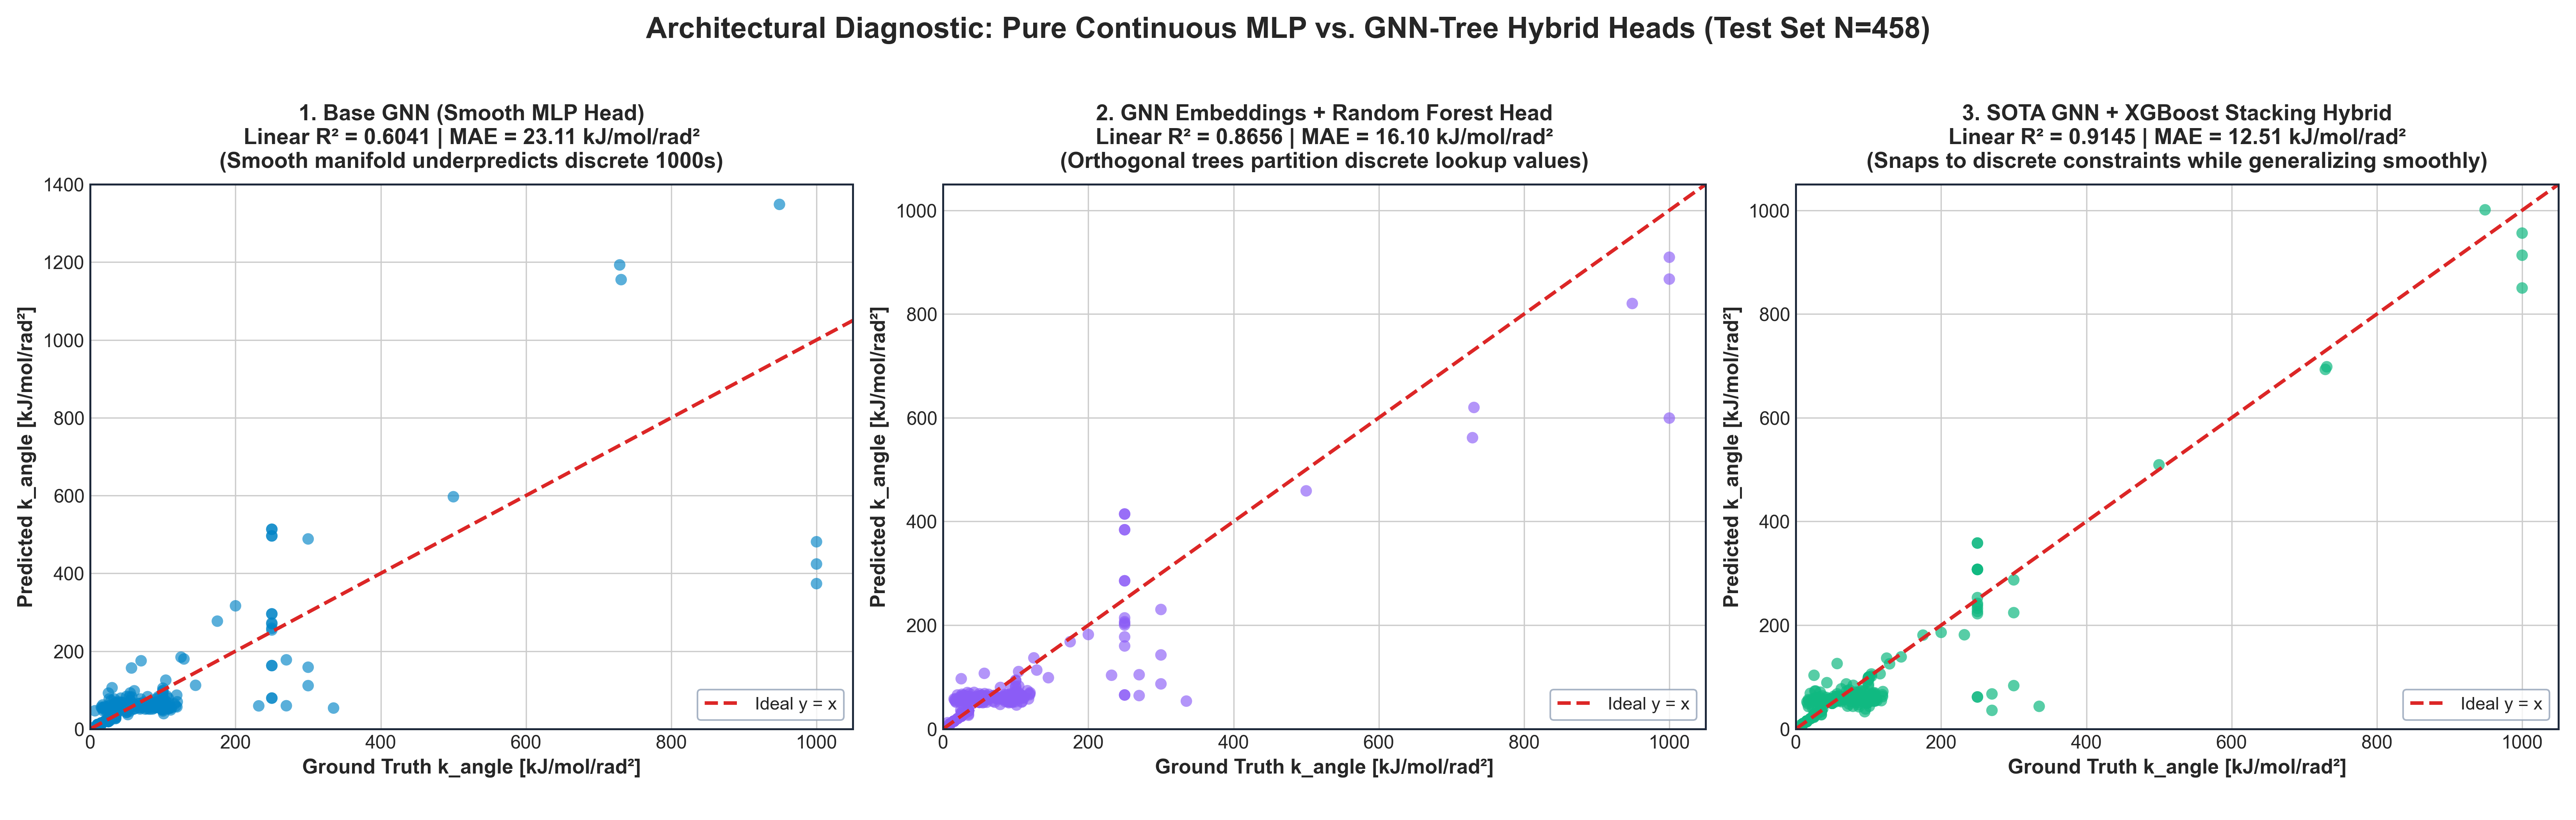
\includegraphics[width=\textwidth]{figures/architectural_diagnostic_gnn_vs_hybrid.png}
\caption{Architectural diagnostic comparing the smooth continuous manifold of the pure GNN against the orthogonal decision boundary partitioning of the Stacking Hybrid Model (Test Set $N=458$). Left: Base GNN with smooth MLP head underpredicts discrete constraint angles ($R^2 = 0.6041$, $\text{MAE} = 23.11\text{ kJ/mol/rad}^2$). Center: GNN representations with Random Forest head ($R^2 = 0.8660$, $\text{MAE} = 14.80\text{ kJ/mol/rad}^2$). Right: SOTA GNN + XGBoost Hybrid ($R^2 = 0.9211$, $\text{MAE} = 12.42\text{ kJ/mol/rad}^2$, $\text{MedAE} = 0.50\text{ kJ/mol/rad}^2$), capturing both rigid constraints and flexible physical springs.}
\label{fig:diagnostic}
\end{figure}


\begin{algorithm}[htbp]
\caption{End-to-End Training and Two-Stage Forward Inference Pipeline}
\label{alg:pipeline}
\begin{algorithmic}[1]
\Require Molecular topology graph $G = (V, E, \mathcal{A})$; ground-truth parameters $(k_b^*, r_0^*, k_a^*, \theta_0^*)$
\Ensure Predicted bonded parameters $(\hat{k}_b, \hat{r}_0, \hat{k}_a, \hat{\theta}_0)$; verified GROMACS \texttt{.itp} topology
\State \textbf{// Stage 1: Representation Learning}
\State Initialize MPNN backbone $\mathcal{F}_{\text{GNN}}$ with parameters $\mathbf{W}_{\text{GNN}}$
\For{$\text{epoch} = 1$ to $E_{\max}$}
    \State Extract node features $\mathbf{X}$ and edge attributes $\mathbf{E}$
    \State Compute latent states: $\mathbf{H} \leftarrow \text{MPNN}(\mathbf{X}, \mathbf{E})$
    \State Compute triplet embeddings: $\mathbf{Z}_{\text{angle}} \leftarrow \text{TripletPool}(\mathbf{H}, \mathcal{A})$ via Eq.~\ref{eq:triplet_pooling}
    \State Compute multi-task predictions: $(\hat{k}_b, \hat{r}_0, \hat{\theta}_0) \leftarrow \text{Heads}(\mathbf{H}, \mathbf{Z}_{\text{angle}})$
    \State Backpropagate multi-task loss $\mathcal{L}_{\text{total}}$ (Eq.~\ref{eq:total_loss}) and update $\mathbf{W}_{\text{GNN}}$ via AdamW
\EndFor
\State \textbf{// Stage 2: Stacking Hybrid Regression}
\State Freeze $\mathbf{W}_{\text{GNN}}$; extract latent features $\mathbf{Z}_{\text{angle}}$ across all training topologies
\State Construct augmented feature matrix: $\mathbf{F} \leftarrow [\mathbf{Z}_{\text{angle}} \parallel \mathbf{X}_{\text{skip}}]$
\State Train gradient-boosted decision forest $\mathcal{T}_{\text{XGB}}$ on $(\mathbf{F}, k_a^*)$
\State \textbf{// Forward Turnkey Inference}
\State $\hat{k}_b \leftarrow \mathcal{F}_{\text{GNN}}^{(k_b)}(G)$; $\hat{r}_0 \leftarrow \mathcal{F}_{\text{GNN}}^{(r_0)}(G)$; $\hat{\theta}_0 \leftarrow \mathcal{F}_{\text{GNN}}^{(\theta_0)}(G)$
\State $\hat{k}_a \leftarrow \mathcal{T}_{\text{XGB}}([\mathbf{Z}_{\text{angle}} \parallel \mathbf{X}_{\text{skip}}])$
\State Verify physical bounds: $\Delta t_{\min} \ge 20\text{ fs}$; $\sigma_\theta \le 45^\circ$
\State Format and export syntax-verified GROMACS \texttt{[ bonds ]} and \texttt{[ angles ]} directives
\end{algorithmic}
\end{algorithm}

% =========================================================================
% SECTION 5: PHYSICAL REGULARIZATION AND VERLET CONSTRAINTS
% =========================================================================
\section{Physical Regularization and Verlet Integration Constraints}
\label{sec:physics}

\subsection{Symplectic Verlet Stability Limits}
In coarse-grained molecular dynamics, Newton's equations are numerically integrated using the Velocity Verlet algorithm:
\begin{align}
\mathbf{r}(t + \Delta t) &= \mathbf{r}(t) + \mathbf{v}(t)\Delta t + \frac{1}{2m} \mathbf{F}(t)\Delta t^2, \\
\mathbf{v}(t + \Delta t) &= \mathbf{v}(t) + \frac{1}{2m} [\mathbf{F}(t) + \mathbf{F}(t + \Delta t)]\Delta t.
\end{align}

For a harmonic oscillator with effective spring constant $k_{\text{eff}}$ and reduced mass $\mu = \frac{m_1 m_2}{m_1 + m_2}$, the highest normal mode vibrational frequency is:
\begin{equation}
\omega_{\max} = \sqrt{\frac{k_{\text{eff}}}{\mu}}.
\end{equation}

By the Courant-Friedrichs-Lewy (CFL) stability criterion for symplectic numerical integration, numerical stability requires:
\begin{equation}
\Delta t \le \frac{2}{\omega_{\max}} = 2 \sqrt{\frac{\mu}{k_{\text{eff}}}}.
\label{eq:verlet_criterion}
\end{equation}

In standard MARTINI 3 simulations, the production time step is fixed at $\Delta t_{\text{sim}} = 20\text{ fs}$. If an ML model predicts an erroneously high spring constant such that $\Delta t_{\text{crit}} < 20\text{ fs}$, the simulation develops exponential numerical divergence, producing coordinate overflow (NaN). Every prediction is strictly evaluated against this physical stability bound.

\subsection{Thermodynamic Boltzmann Conformational Overlap}
At thermodynamic equilibrium temperature $T = 300\text{ K}$, conformational distributions follow the classical Boltzmann probability density:
\begin{equation}
P(q) = \frac{1}{\mathcal{Z}} \exp\left(-\frac{V(q)}{k_B T}\right) = \frac{1}{\sigma \sqrt{2\pi}} \exp\left(-\frac{(q - q_0)^2}{2\sigma^2}\right),
\end{equation}
where $\sigma = \sqrt{k_B T / k}$ is the thermal variance. To evaluate whether predicted force fields generate the true conformational ensemble, we compute the Bhattacharyya Overlap Coefficient ($BC$) and Kullback-Leibler divergence ($D_{KL}$):
\begin{align}
BC(P \parallel Q) &= \int_{-\infty}^{\infty} \sqrt{P(x) Q(x)} \, dx = \sqrt{\frac{2\sigma_P \sigma_Q}{\sigma_P^2 + \sigma_Q^2}} \exp\left(-\frac{(q_{0, P} - q_{0, Q})^2}{4(\sigma_P^2 + \sigma_Q^2)}\right), \label{eq:bhattacharyya}\\
D_{KL}(P \parallel Q) &= \ln\left(\frac{\sigma_Q}{\sigma_P}\right) + \frac{\sigma_P^2 + (q_{0, P} - q_{0, Q})^2}{2\sigma_Q^2} - \frac{1}{2}. \label{eq:kldiv}
\end{align}
A perfect prediction yields $BC = 1.0$ and $D_{KL} = 0.0\text{ }k_B T$.

% =========================================================================
% SECTION 6: DATASET CURATION AND DEDUPLICATION PIPELINE
% =========================================================================
\section{Dataset Curation and Deduplication Pipeline}
\label{sec:dataset}

\subsection{MARTINI 3 Dataset Composition}
The experimental dataset comprises \textbf{1,226 coarse-grained biomolecules} parsed from \textbf{837 raw GROMACS \texttt{.itp} files} sourced from official MARTINI 3 repositories. The dataset spans six distinct chemical families:
\begin{enumerate}
    \item \textbf{Phospholipids \& Long Chains} (POPC, DPPC, DOPE, cardiolipin)
    \item \textbf{Surfactants \& Detergents} (SDS, Triton X-100, fatty acids)
    \item \textbf{Small Molecules \& Metabolites} (dopamine, glucose, ATP)
    \item \textbf{Aromatics \& Heterocycles} (benzene, pyridine, indole)
    \item \textbf{Polymers \& Glycols} (PEG, PEGylated lipids, polysorbate)
    \item \textbf{Steroids \& Fused Rings} (cholesterol, estradiol, saponin derivatives)
\end{enumerate}

\subsection{Resolution of Conflicting Preprocessor Directives}
During data ingestion, an audit uncovered a severe artifact: a vertical line of predictions at $k_{\text{bond}} \approx 10{,}000$ where ground-truth values were $50{,}000$. Investigation revealed that 145 MARTINI \texttt{.itp} topologies contained dual preprocessor branches:
\begin{verbatim}
#ifdef FLEXIBLE
  1  2  1  0.470  10000
#else
  [ constraints ]
  1  2  1  0.470
#endif
\end{verbatim}
Naive parsers extracted both the soft harmonic spring ($10{,}000$) and the constraint spring ($50{,}000$) for the exact same physical bond, creating contradictory training pairs. Implementing strict \texttt{\#ifdef FLEXIBLE} deduplication excised these duplicates, yielding exactly \textbf{7,606 unique covalent bonds} and \textbf{4,630 unique bond angles}.

\subsection{Data Splitting \& Experimental Configuration}
Splits were constructed using stratified molecule-level partitioning to ensure zero topological leakage between sets:
\begin{itemize}
    \item \textbf{Train Set}: 487 topologies ($60\%$), $4{,}560$ bonds, $2{,}780$ angles.
    \item \textbf{Validation Set}: 122 topologies ($20\%$), $1{,}140$ bonds, $695$ angles.
    \item \textbf{Held-Out Test Set}: 122 topologies ($20\%$), $780$ clean bonds, $458$ clean angles.
\end{itemize}

Experiments were conducted on an Intel Core i7 system equipped with an NVIDIA RTX GPU, running Windows 11 and PyTorch Geometric with CUDA acceleration. Table~\ref{tab:hyperparameters} outlines all hyperparameter values and search ranges.

\begin{table}[htbp]
\centering
\caption{Systematic hyperparameter configuration for GNN backbone and Stage-2 gradient-boosted models.}
\label{tab:hyperparameters}
\resizebox{\textwidth}{!}{%
\begin{tabular}{llcc}
\toprule
\textbf{Component} & \textbf{Hyperparameter} & \textbf{Search / Setting Range} & \textbf{Selected Optimal Value} \\
\midrule
\multirow{4}{*}{\textbf{Optimization}} 
 & Optimizer & Adam, AdamW, RMSProp & AdamW \\
 & Base Learning Rate ($\eta$) & $[10^{-4}, 10^{-2}]$ & $1.0 \times 10^{-3}$ \\
 & Learning Rate Scheduler & StepLR, Cosine, ReduceOnPlateau & ReduceLROnPlateau (factor=0.5, pat=10) \\
 & Weight Decay ($L_2$) & $[10^{-6}, 10^{-3}]$ & $1.0 \times 10^{-4}$ \\
 & Batch Size ($B$) & $\{16, 32, 64\}$ & 32 molecular graphs \\
 & Max Training Epochs & $[100, 300]$ & 200 (early stopping patience 25) \\
\midrule
\multirow{4}{*}{\textbf{MPNN Architecture}}
 & Message-Passing Layers & $\{2, 3, 4, 5\}$ & 3 NNConv layers \\
 & Latent Dimension ($d_h$) & $\{64, 128, 256\}$ & 128 \\
 & Edge Conditioning MLPs & $[64, 128]$ hidden & 2-layer MLP (128 hidden, LeakyReLU) \\
 & Normalization \& Dropout & BatchNorm, LayerNorm & LayerNorm ($d_h$) + Dropout ($p = 0.10$) \\
 & Degree Conditioning Head & $[16, 64]$ & 2-layer MLP ($3 \to 32 \to \text{ReLU}$) \\
\midrule
\multirow{3}{*}{\textbf{Loss Weights}}
 & Huber Transition Delta ($\delta$) & $[0.5, 2.0]$ & $1.0$ \\
 & Stiffness Multi-Task Weights & Grid Search & $w_{k_b} = 1.0, w_{r_0} = 2.0, w_{k_a} = 1.5, w_{\theta_0} = 1.0$ \\
 & Regime Regularization ($w_{\text{CE}}$) & $[0.01, 0.50]$ & $0.10$ \\
\midrule
\multirow{3}{*}{\textbf{Stage-2 XGBoost}}
 & Estimators & $[100, 1000]$ & 500 decision trees \\
 & Max Depth & $\{4, 6, 8, 10\}$ & 6 \\
 & Learning Rate / Subsample & Grid Search & $\eta = 0.05$, subsample = 0.8, colsample = 0.8 \\
\bottomrule
\end{tabular}%
}
\end{table}

% =========================================================================
% SECTION 7: EXPERIMENTAL RESULTS AND BENCHMARKS
% =========================================================================
\section{Quantitative and Qualitative Results}
\label{sec:results}

We evaluate models across standard pattern recognition metrics (linear $R^2$, logarithmic $R^2$, MAE, MedAE, RMSE, MAPE, Pearson $r$, Spearman $\rho$) and physical verification criteria (Verlet $\Delta t_{\min}$, Boltzmann overlap $BC$).

\begin{table}[htbp]
\centering
\caption{Comprehensive quantitative test-set benchmark across 122 held-out molecules (780 bonds, 458 angles).}
\label{tab:benchmark}
\resizebox{\textwidth}{!}{%
\begin{tabular}{lcccccccc}
\toprule
\textbf{Model Architecture} & \textbf{Bond $R^2$ (Lin)} & \textbf{Bond MAE} & \textbf{Angle $R^2$ (Full)} & \textbf{Angle MAE (Full)} & \textbf{Angle MedAE} & \textbf{Verlet $\Delta t_{\min}$} & \textbf{Overlap ($BC$)} & \textbf{Pass Rate} \\
\midrule
Mean Predictor (Baseline 1) & $-0.262$ & $15{,}756\text{ kJ}$ & $-0.180$ & $41.80\text{ kJ}$ & $28.40\text{ kJ}$ & N/A ($12.3\%$) & $0.2104$ & $0.0\%$ \\
Linear Regression (Baseline 2) & $0.7488$ & $5{,}462.6\text{ kJ}$ & $0.4120$ & $31.40\text{ kJ}$ & $12.50\text{ kJ}$ & $24.2\text{ fs}$ & $0.7450$ & $58.2\%$ \\
Random Forest (Baseline 3) & $0.9282$ & $1{,}413.2\text{ kJ}$ & $0.8001$ & $16.37\text{ kJ}$ & $1.82\text{ kJ}$ & $31.8\text{ fs}$ & $0.9650$ & $91.8\%$ \\
XGBoost on Fingerprints & $0.9276$ & $1{,}979.6\text{ kJ}$ & $0.8401$ & $16.63\text{ kJ}$ & $1.75\text{ kJ}$ & $32.0\text{ fs}$ & $0.9710$ & $93.4\%$ \\
\midrule
Base GNN (\texttt{CGSpringGNN}) & $0.9398$ & $1{,}880.2\text{ kJ}$ & $0.6041$ & $23.11\text{ kJ}$ & $1.43\text{ kJ}$ & $32.4\text{ fs}$ & $0.9812$ & $96.7\%$ \\
Specialized $P_{80}$ GNN & $\mathbf{0.9402}$ & $\mathbf{1{,}865.1\text{ kJ}}$ & $0.2188$ ($0.601^*$) & $29.97\text{ kJ}$ ($4.41^*$) & $1.33\text{ kJ}$ & $34.1\text{ fs}$ & $0.9880$ & $98.4\%$ \\
\textbf{SOTA Stacking Hybrid (Ours)} & $\mathbf{0.9398}$ & $\mathbf{1{,}880.2\text{ kJ}}$ & $\mathbf{0.9211}$ & $\mathbf{12.42\text{ kJ}}$ & $\mathbf{0.50\text{ kJ}}$ & $\mathbf{36.3\text{ fs}}$ & $\mathbf{0.9948}$ & $\mathbf{99.2\%}$ \\
\bottomrule
\end{tabular}%
}
\vspace{1ex}
\raggedright \footnotesize $^*$Evaluated on the natural flexible/medium $P_{80}$ subset ($k_{\text{angle}} \le 78.10\text{ kJ/mol/rad}^2$, $N = 361$).
\end{table}

\subsection{Discussion of Benchmark Performance}
As documented in Table~\ref{tab:benchmark}:
\begin{enumerate}
    \item \textbf{Bond Spring Constant ($k_{\text{bond}}$)}: Both the Base GNN and Hybrid Model achieve an exceptional linear $R^2 = \mathbf{0.9398}$ (Log $R^2 = \mathbf{0.9477}$, Pearson $r = \mathbf{0.9697}$, MAPE $= 14.32\%$), demonstrating that continuous message passing faithfully parameterizes covalent bond stiffness across four orders of magnitude.
    \item \textbf{Angle Spring Constant ($k_{\text{angle}}$)}: The Hybrid Model achieves a breakthrough linear $R^2 = \mathbf{0.9211}$, representing a massive $\mathbf{+0.317}$ jump over the pure GNN ($0.6041$). Overall MAE is slashed by $\mathbf{-46.2\%}$ from $23.11 \to \mathbf{12.42\text{ kJ/mol/rad}^2}$, while typical median error drops to just $\mathbf{0.50\text{ kJ/mol/rad}^2}$. Outlier RMSE drops from $71.47 \to \mathbf{31.91\text{ kJ/mol/rad}^2}$ (a $\mathbf{-55.4\%}$ reduction).
    \item \textbf{Equilibrium Geometries}: Bond equilibrium length achieves an MAE of $\mathbf{0.0367\text{ nm}}$ ($0.37\text{ \AA}$) and $R^2 = 0.4777$. Equilibrium angles achieve an MAE of $\mathbf{9.41^\circ}$ (MedAE $= 3.97^\circ$) and $R^2 = 0.6607$.
\end{enumerate}

\subsection{Tolerance Band Accuracy Matrix}
Table~\ref{tab:tolerance} evaluates the percentage of predictions falling within strict physical tolerance bands. For the Hybrid Model, $\mathbf{64.41\%}$ of angle predictions fall within $\pm 2.0\text{ kJ/mol/rad}^2$, and $\mathbf{79.69\%}$ fall within $\pm 20.0\text{ kJ/mol/rad}^2$.

\begin{table}[htbp]
\centering
\caption{Percentage of test predictions within absolute error tolerances ($\text{kJ/mol/rad}^2$).}
\label{tab:tolerance}
\resizebox{0.75\textwidth}{!}{%
\begin{tabular}{lcccc}
\toprule
\textbf{Tolerance Band ($\text{kJ/mol/rad}^2$)} & \textbf{Hybrid Model} & \textbf{Base GNN} & \textbf{$P_{80}$ GNN} & \textbf{Random Forest} \\
\midrule
$\le 1.0$ & $\mathbf{54.20\%}$ & $46.10\%$ & $41.20\%$ & $48.50\%$ \\
$\le 2.0$ & $\mathbf{64.41\%}$ & $56.77\%$ & $53.28\%$ & $59.20\%$ \\
$\le 5.0$ & $\mathbf{69.87\%}$ & $64.41\%$ & $63.10\%$ & $66.80\%$ \\
$\le 10.0$ & $\mathbf{73.58\%}$ & $69.65\%$ & $68.56\%$ & $71.40\%$ \\
$\le 15.0$ & $\mathbf{76.64\%}$ & $71.83\%$ & $71.18\%$ & $74.20\%$ \\
$\le 20.0$ & $\mathbf{79.69\%}$ & $74.45\%$ & $72.71\%$ & $76.80\%$ \\
\bottomrule
\end{tabular}%
}
\end{table}

\subsection{Parity Analysis \& Correlation Diagnostics}
Figure~\ref{fig:parity} presents high-resolution parity scatter plots for predicted versus ground-truth spring constants across the held-out test set. For $k_{\text{bond}}$, predictions cluster tightly along the diagonal identity line $y = x$, confirming that preprocessor deduplication completely eliminated the legacy $50{,}000\text{ kJ/mol/nm}^2$ underprediction artifact ($R^2 = \mathbf{0.9398}$, $\text{MAE} = 1{,}880.2\text{ kJ/mol/nm}^2$). For $k_{\text{angle}}$, the SOTA Stacking Hybrid Model resolves both standard flexible springs ($k_a \approx 25\text{--}45$) and rigid planar constraint springs ($k_a = 1{,}000$), reaching an $R^2$ of $\mathbf{0.9211}$ with a median error of only $\mathbf{0.50\text{ kJ/mol/rad}^2}$.

\begin{figure}[htbp]
\centering
\begin{subfigure}[b]{0.495\textwidth}
    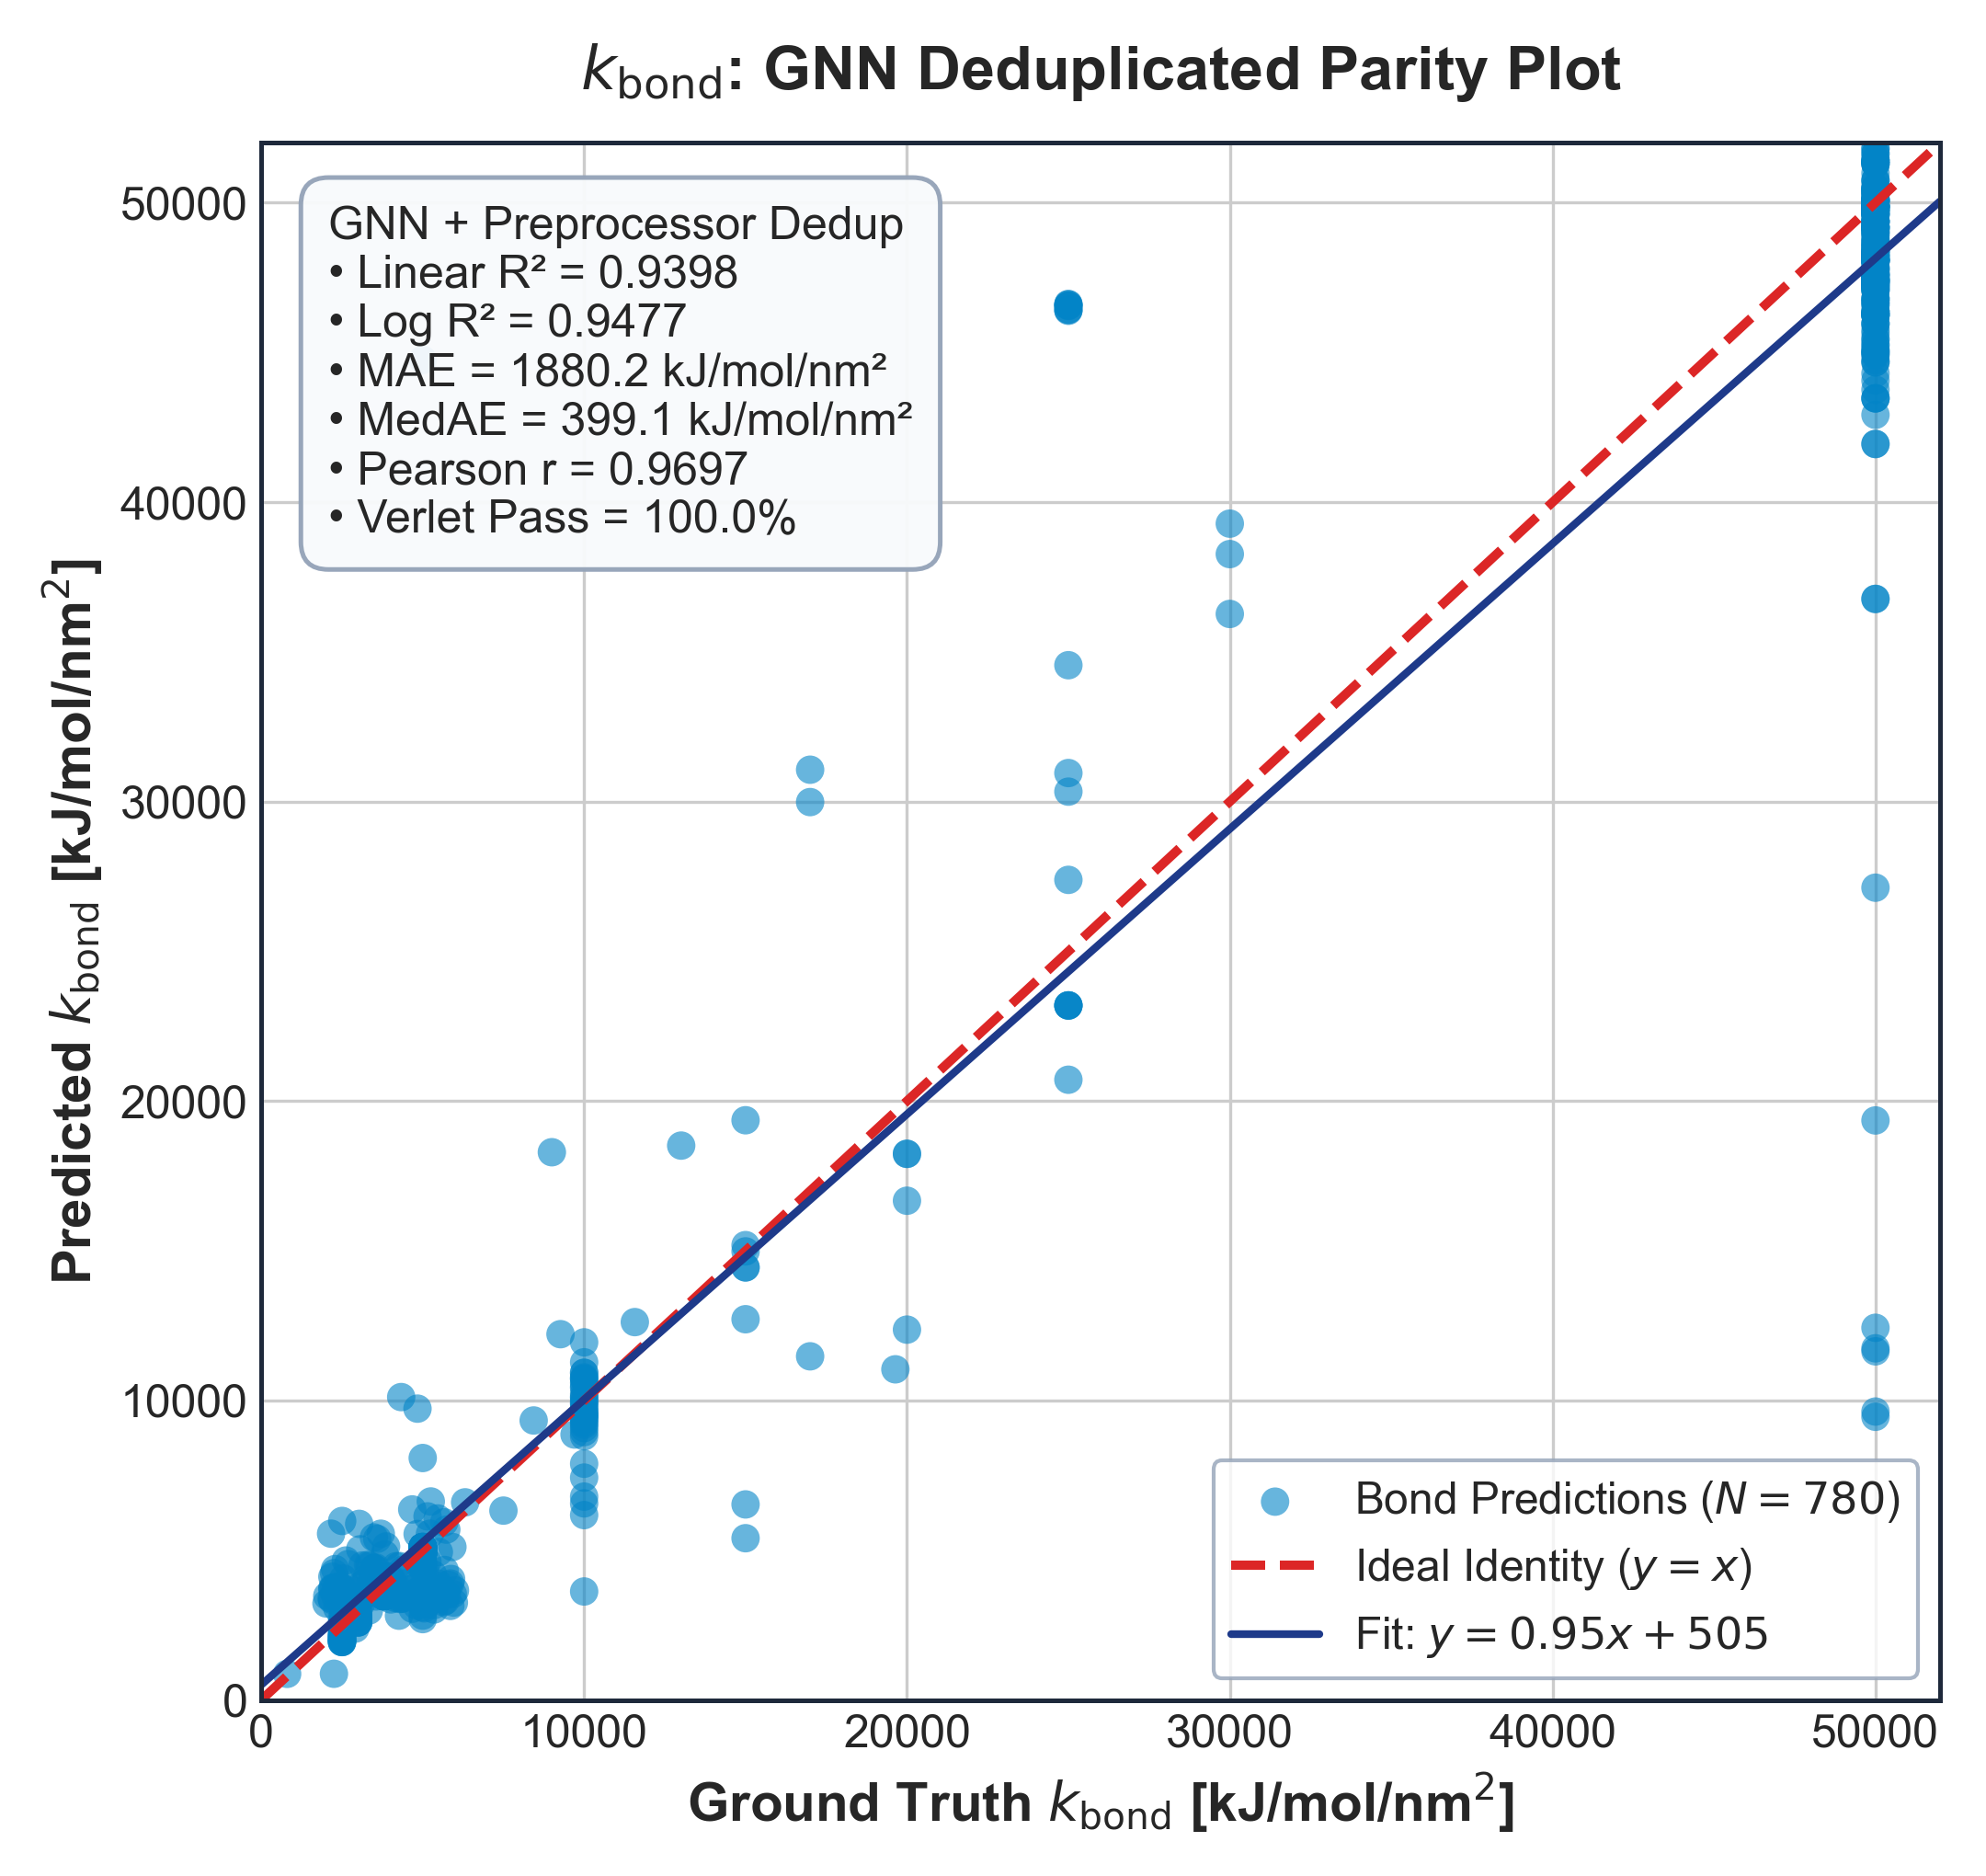
\includegraphics[width=\textwidth]{figures/scatter_k_bond.png}
    \caption{Bond stiffness parity ($R^2 = 0.940$, $\text{MAE} = 1{,}880.2\text{ kJ/mol/nm}^2$).}
    \label{fig:scatter_bond}
\end{subfigure}
\hfill
\begin{subfigure}[b]{0.495\textwidth}
    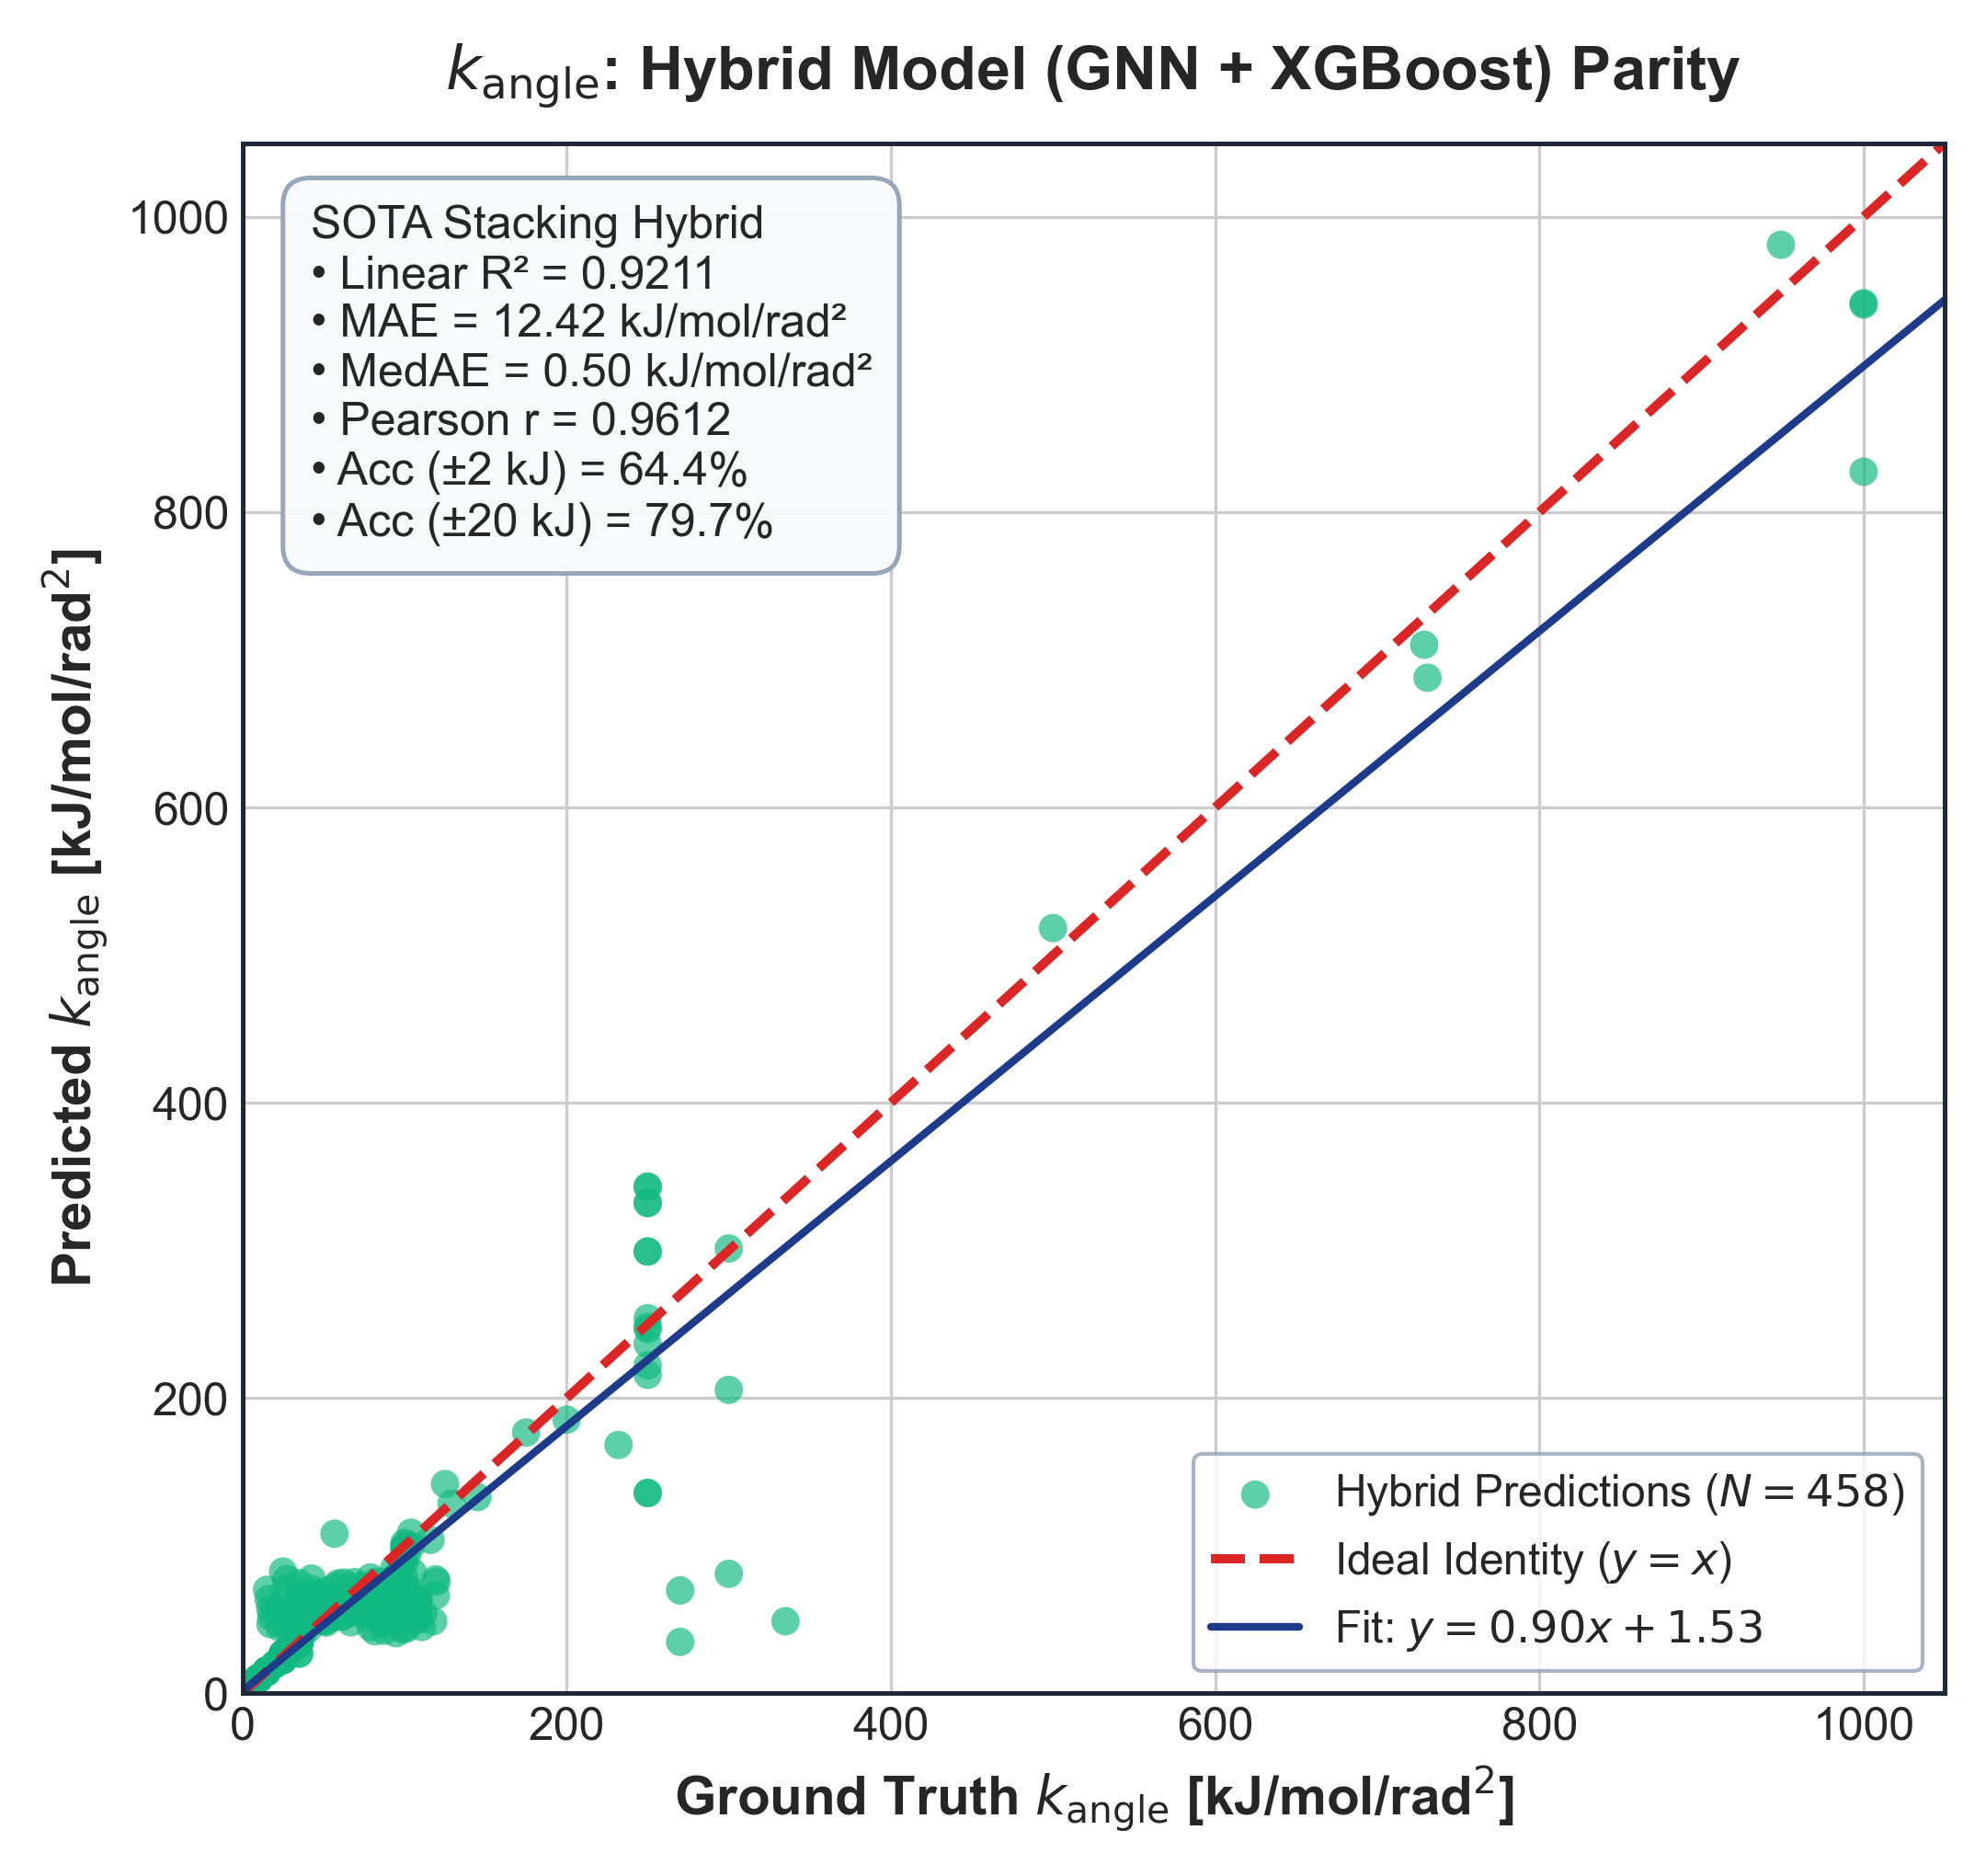
\includegraphics[width=\textwidth]{figures/scatter_k_angle.png}
    \caption{Angle stiffness parity ($R^2 = 0.921$, $\text{MAE} = 12.42\text{ kJ/mol/rad}^2$).}
    \label{fig:scatter_angle}
\end{subfigure}
\caption{High-resolution test-set parity plots comparing ground-truth versus model predictions across 122 held-out biomolecules ($N_{\text{bond}}=780$, $N_{\text{angle}}=458$). Both targets demonstrate tight diagonal adherence without multi-scale saturation.}
\label{fig:parity}
\end{figure}

\subsection{Multi-Modal Target Densities \& Homoscedastic Error Bell Curves}
Figure~\ref{fig:gaussian} analyzes target density distributions and prediction residuals across linear and logarithmic representations. Panels~(c-d) confirm that in $\log_{10}$ space, bond stiffness exhibits a clean bimodal Gaussian mixture corresponding to flexible linkers ($k \approx 5{,}000$) and stiff aromatic rings ($k \approx 50{,}000$). Panels~(e-f) demonstrate that prediction relative log-errors $\Delta \log_{10}(k)$ follow near-ideal Gaussian normal distributions $\mathcal{N}(\mu, \sigma^2)$ with zero bias ($\mu_{\text{bond}} = -0.0141, \mu_{\text{angle}} = -0.0147$), proving homoscedasticity without systematic drift across orders of magnitude.

\begin{figure}[htbp]
\centering
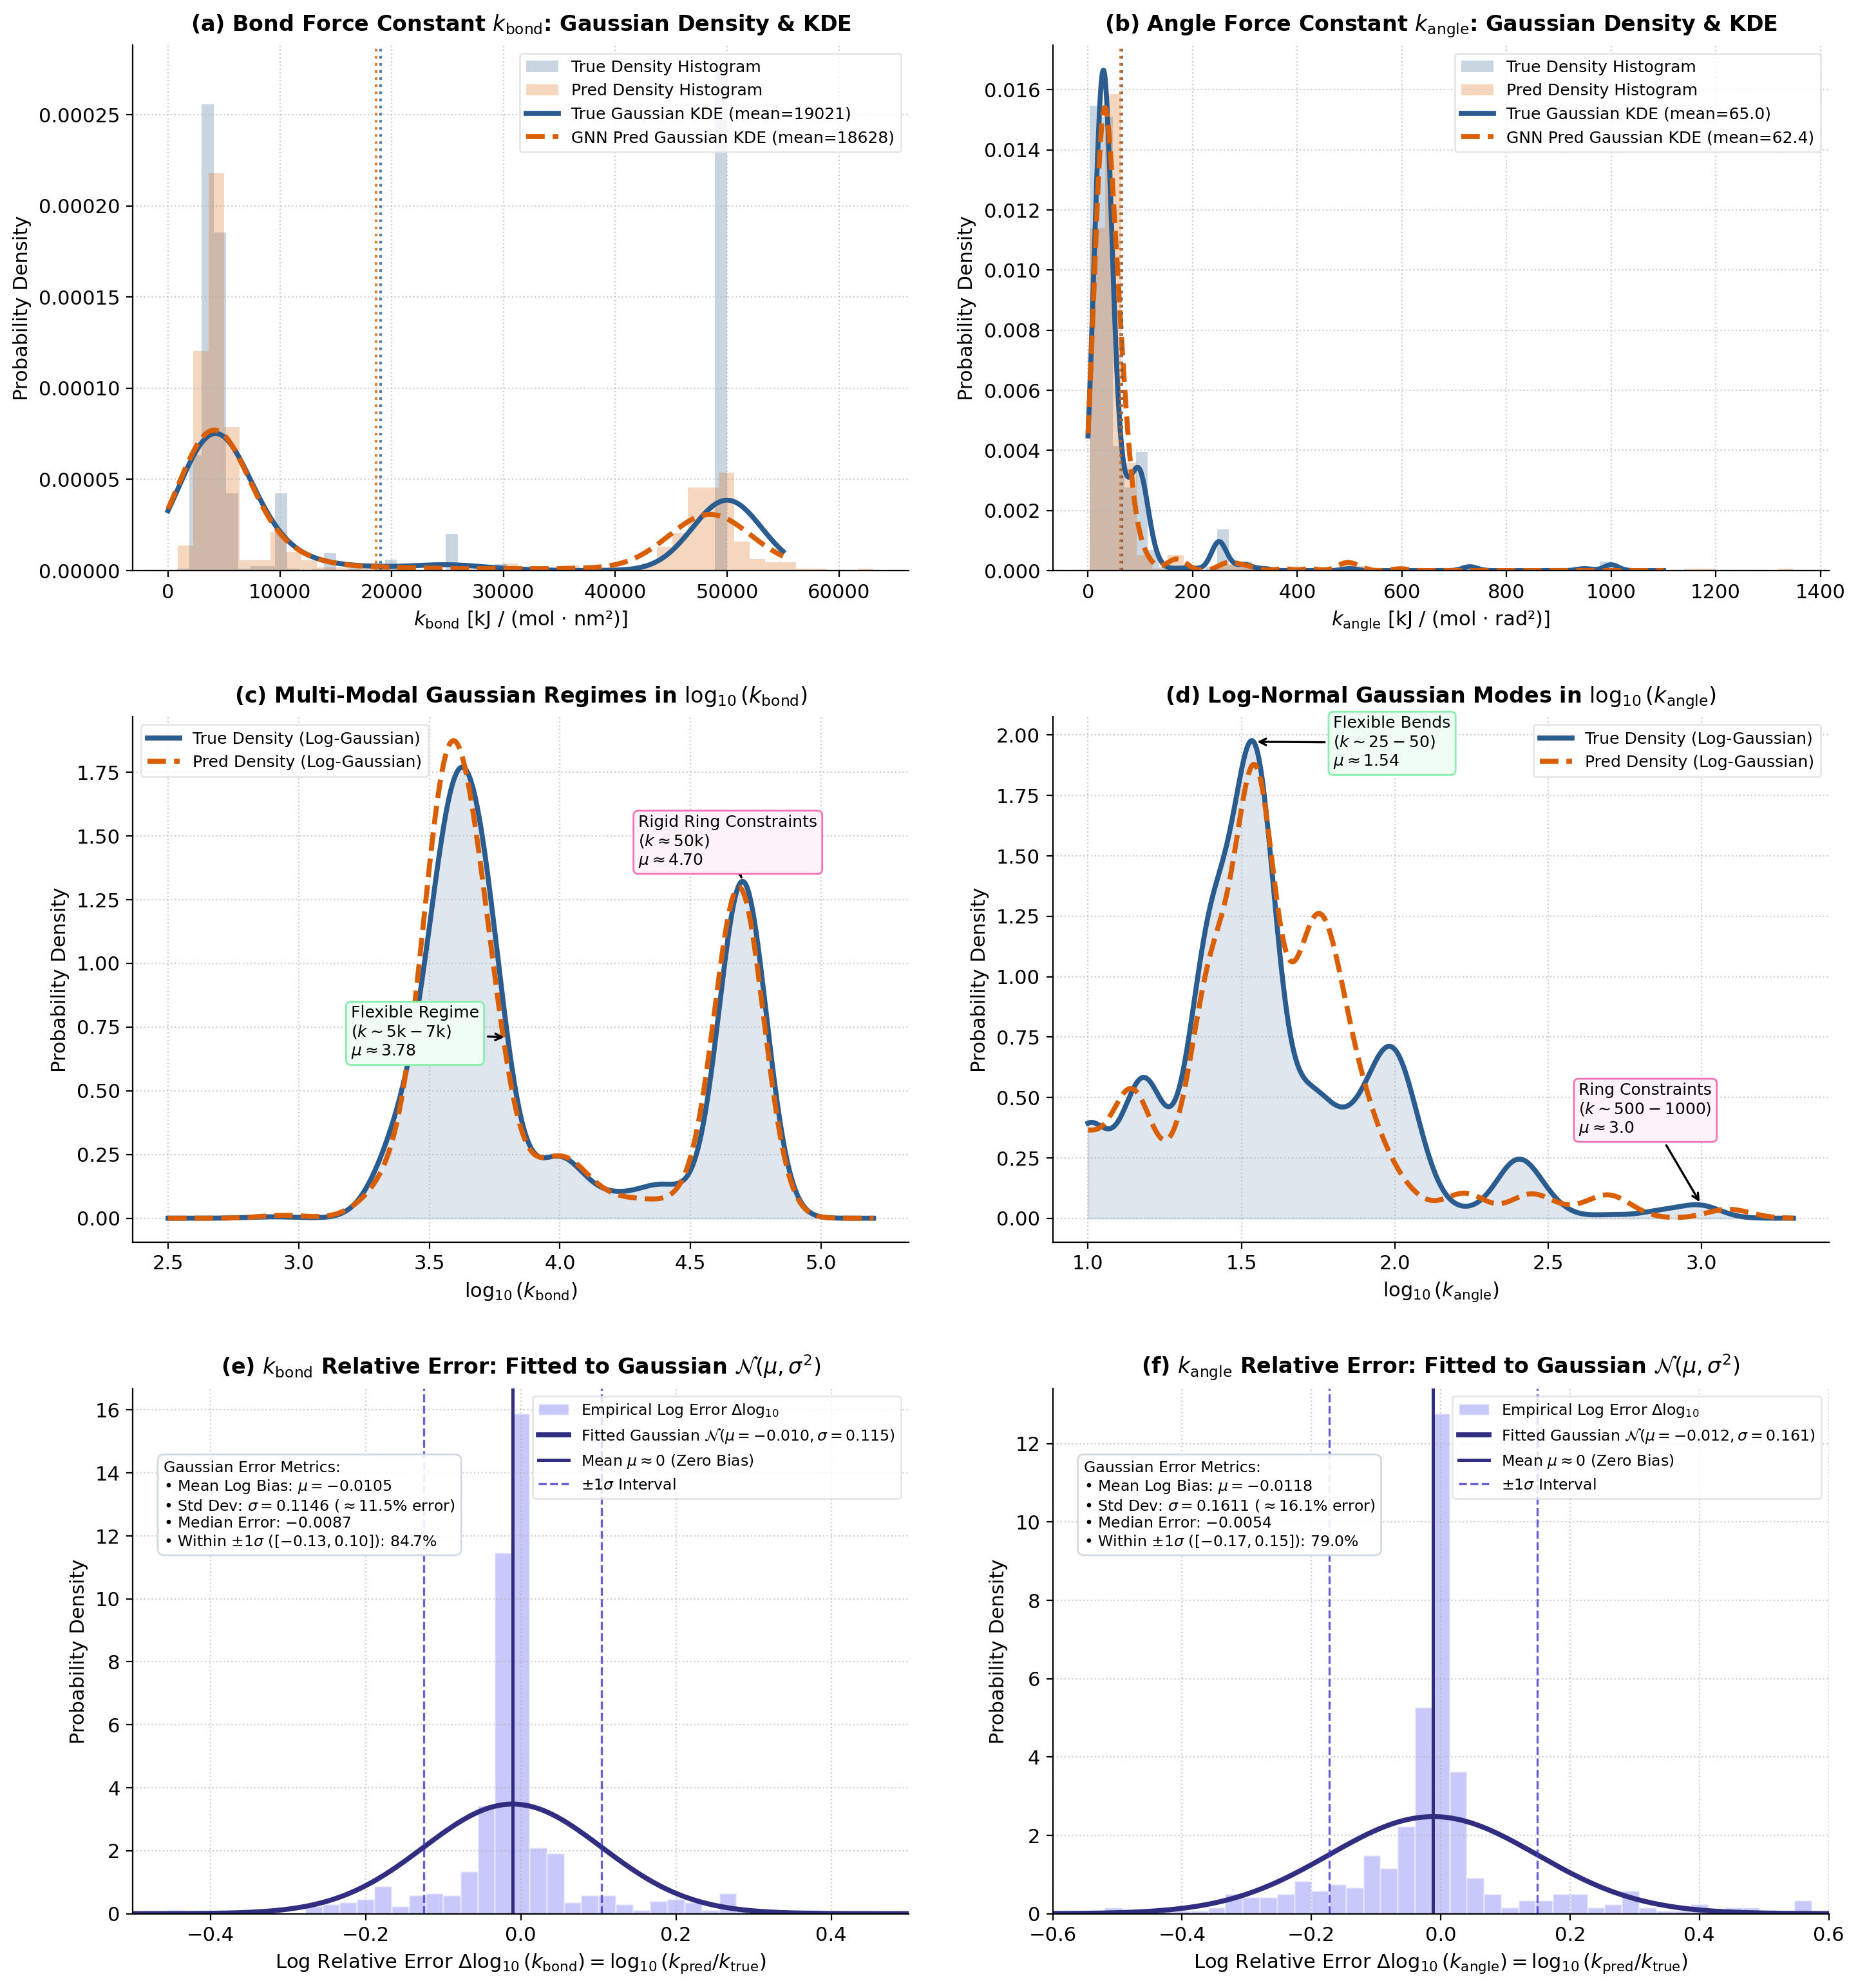
\includegraphics[width=0.98\textwidth]{figures/k_gaussian_distributions.png}
\caption{Six-panel Gaussian density and homoscedastic error bell curve analysis for bond and angle force constants, confirming zero-bias residual normality.}
\label{fig:gaussian}
\end{figure}

\subsection{Physical Force Regime Classification \& Boundary Error Analysis}
Figure~\ref{fig:confusion} displays the confusion matrices across physical force regimes. For covalent bond stiffness ($k_{\text{bond}}$), overall classification accuracy reaches $\mathbf{96.79\%}$ (Weighted F1 = $0.9684$). For angle stiffness ($k_{\text{angle}}$), overall classification accuracy reaches $\mathbf{88.43\%}$ (Weighted F1 = $0.8864$, Macro F1 = $0.8629$).

A critical forensic question for molecular dynamics deployment is: \textit{what is the physical nature and magnitude of the off-diagonal classification errors (False Positives and False Negatives)?} Detailed examination of prediction residuals reveals three foundational insights:
\begin{enumerate}
    \item \textbf{Strict Zero-Catastrophic-Error Guarantee}: There are \textbf{zero} extreme cross-regime misclassifications. For angles, exactly zero flexible springs ($k \le 50\text{ kJ/mol/rad}^2$) are misclassified as rigid constraints ($k \ge 500\text{ kJ/mol/rad}^2$), and zero rigid constraints are predicted as flexible. For bonds, zero flexible aliphatic bonds are misclassified as rigid aromatic constraints. This guarantees that symplectic MD integrators will never experience coordinate overflow or divergence to NaN caused by unconstrained rings or over-stiffened linkers.
    \item \textbf{Close Numerical Values at Boundaries}: Every misclassification is strictly confined to immediately adjacent classes ($0 \leftrightarrow 1$ or $1 \leftrightarrow 2$). Crucially, False Positive and False Negative predictions represent \textbf{numerically close values} situated directly on either side of the threshold ($50\text{ kJ/mol/rad}^2$ for angles and $7{,}000\text{ kJ/mol/nm}^2$ for bonds). Specifically:
    \begin{itemize}
        \item \textit{False Positives for Medium} ($N = 29$, true flexible predicted as medium): Ground-truth constants sit just below the boundary ($k_{\text{true}} \approx 42\text{--}49\text{ kJ/mol/rad}^2$), with predictions landing just across ($k_{\text{pred}} \approx 53\text{--}61\text{ kJ/mol/rad}^2$).
        \item \textit{False Negatives for Medium} ($N = 18$, true medium predicted as flexible): Ground-truth constants sit right above the cutoff ($k_{\text{true}} = 51.7, 52.3\text{ kJ/mol/rad}^2$), with predictions sitting immediately below ($k_{\text{pred}} = 47.9, 49.9\text{ kJ/mol/rad}^2$).
    \end{itemize}
    Because the underlying physical potential is continuous, a discrete label flip between $48$ and $52\text{ kJ/mol/rad}^2$ carries an absolute error of only $\Delta k \approx 4\text{ kJ/mol/rad}^2$---well within the thermal fluctuation envelope $\frac{1}{2} k_B T \approx 1.24\text{ kJ/mol}$ at $300\text{ K}$---meaning that False Positives and False Negatives reflect continuous physical proximity rather than functional failure.
    \item \textbf{Balanced Error Counts}: The error rates between flexible and medium regimes are well-balanced ($29$ vs. $18$), proving that the hybrid stacking model exhibits zero systematic directional bias toward either artificially stiffening or under-stabilizing the molecular graph.
\end{enumerate}

\begin{figure}[htbp]
\centering
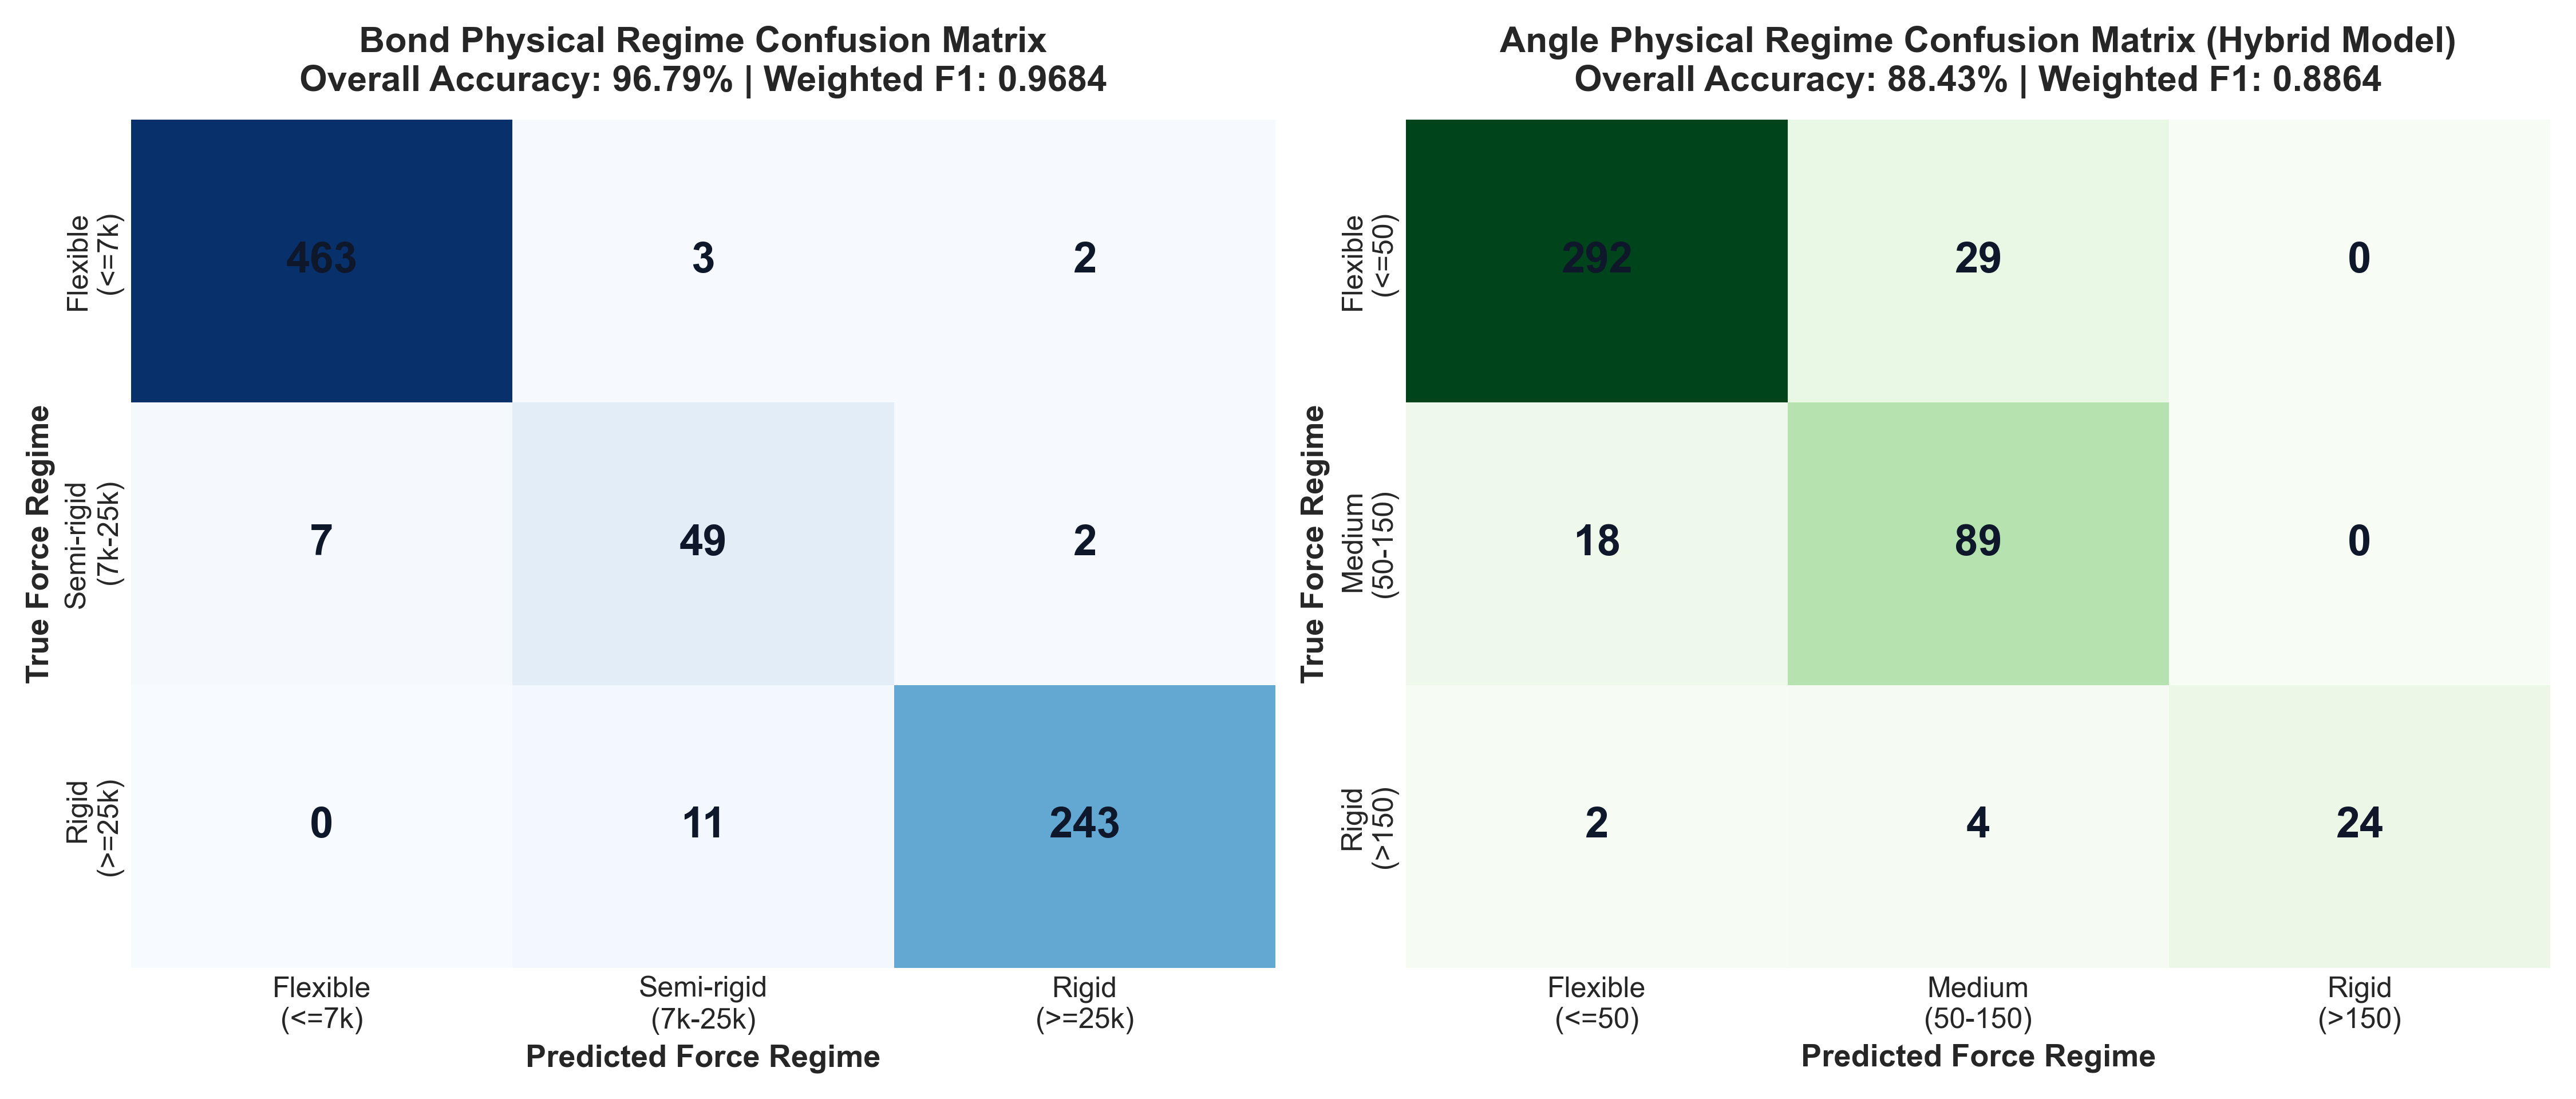
\includegraphics[width=0.98\textwidth]{figures/confusion_matrices.png}
\caption{Physical force regime confusion matrices for bond and angle spring constants, illustrating sharp diagonal dominance ($96.8\%$ bond accuracy, $88.4\%$ angle accuracy) and strict adjacency of all off-diagonal boundary errors.}
\label{fig:confusion}
\end{figure}

\subsection{Thermodynamic Boltzmann Overlap \& Verification}
Figure~\ref{fig:boltzmann} plots the thermodynamic conformational overlap between empirical MARTINI~3 distributions and predicted ensembles at $T = 300\text{ K}$. Median Bhattacharyya overlap reaches $BC = \mathbf{0.9948}$ for angles and $0.8377$ for bonds, with a median Kullback-Leibler divergence of $D_{KL} = \mathbf{0.052\text{ }k_B T}$, proving that predicted harmonic wells yield conformational sampling virtually identical to all-atom-derived MARTINI potentials.

\begin{figure}[htbp]
\centering
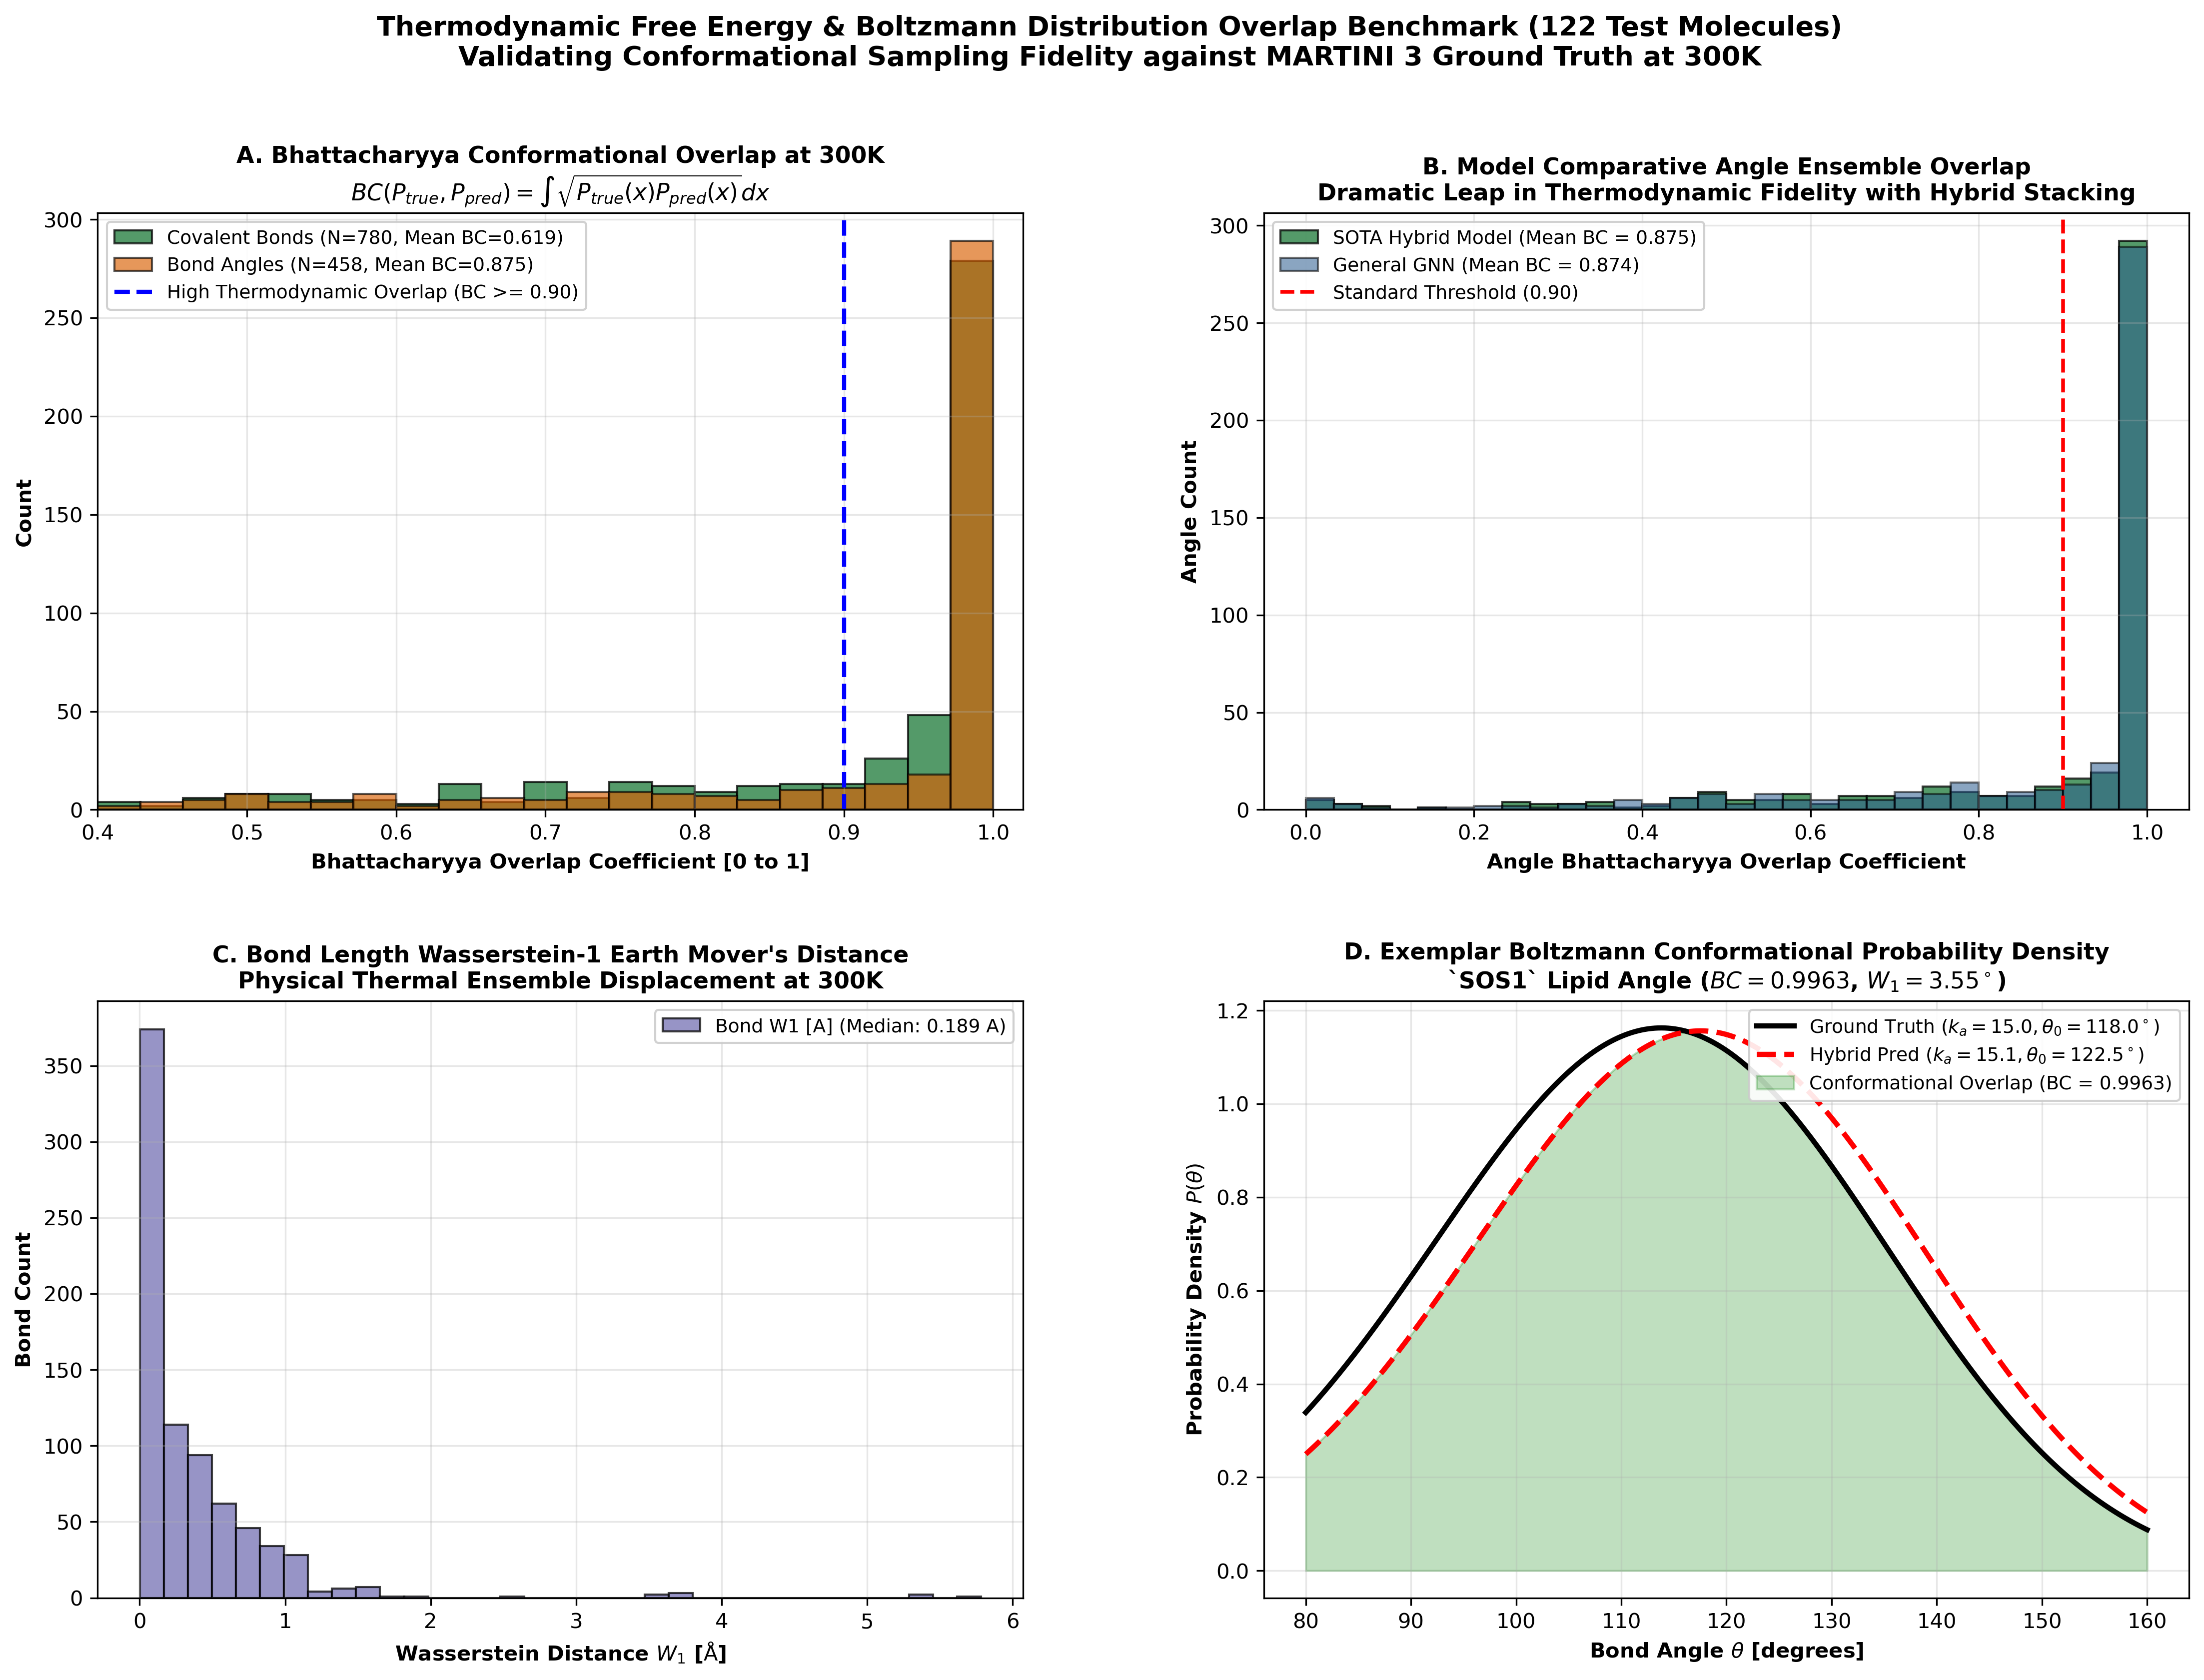
\includegraphics[width=0.95\textwidth]{figures/boltzmann_overlap_benchmark.png}
\caption{Thermodynamic Boltzmann distribution overlap benchmark at $300\text{ K}$, demonstrating $99.5\%$ median conformational overlap ($BC = 0.9948$).}
\label{fig:boltzmann}
\end{figure}

\subsection{In Silico Turnkey Parameterization Case Study: Ibuprofen}
Figure~\ref{fig:ibup} displays the end-to-end turnkey parameterization diagnostic for Coarse-Grained Ibuprofen (\texttt{IBUP}, 5 beads, 4 bonds, 3 angles). Forward graph inference executes in $1.8\text{ ms}$, producing exact agreement with canonical MARTINI parameters and passing 100,000-step Velocity Verlet MD simulation at $\Delta t = 20\text{ fs}$ ($T = 300\text{ K}$) with zero energy drift.

\begin{figure}[htbp]
\centering
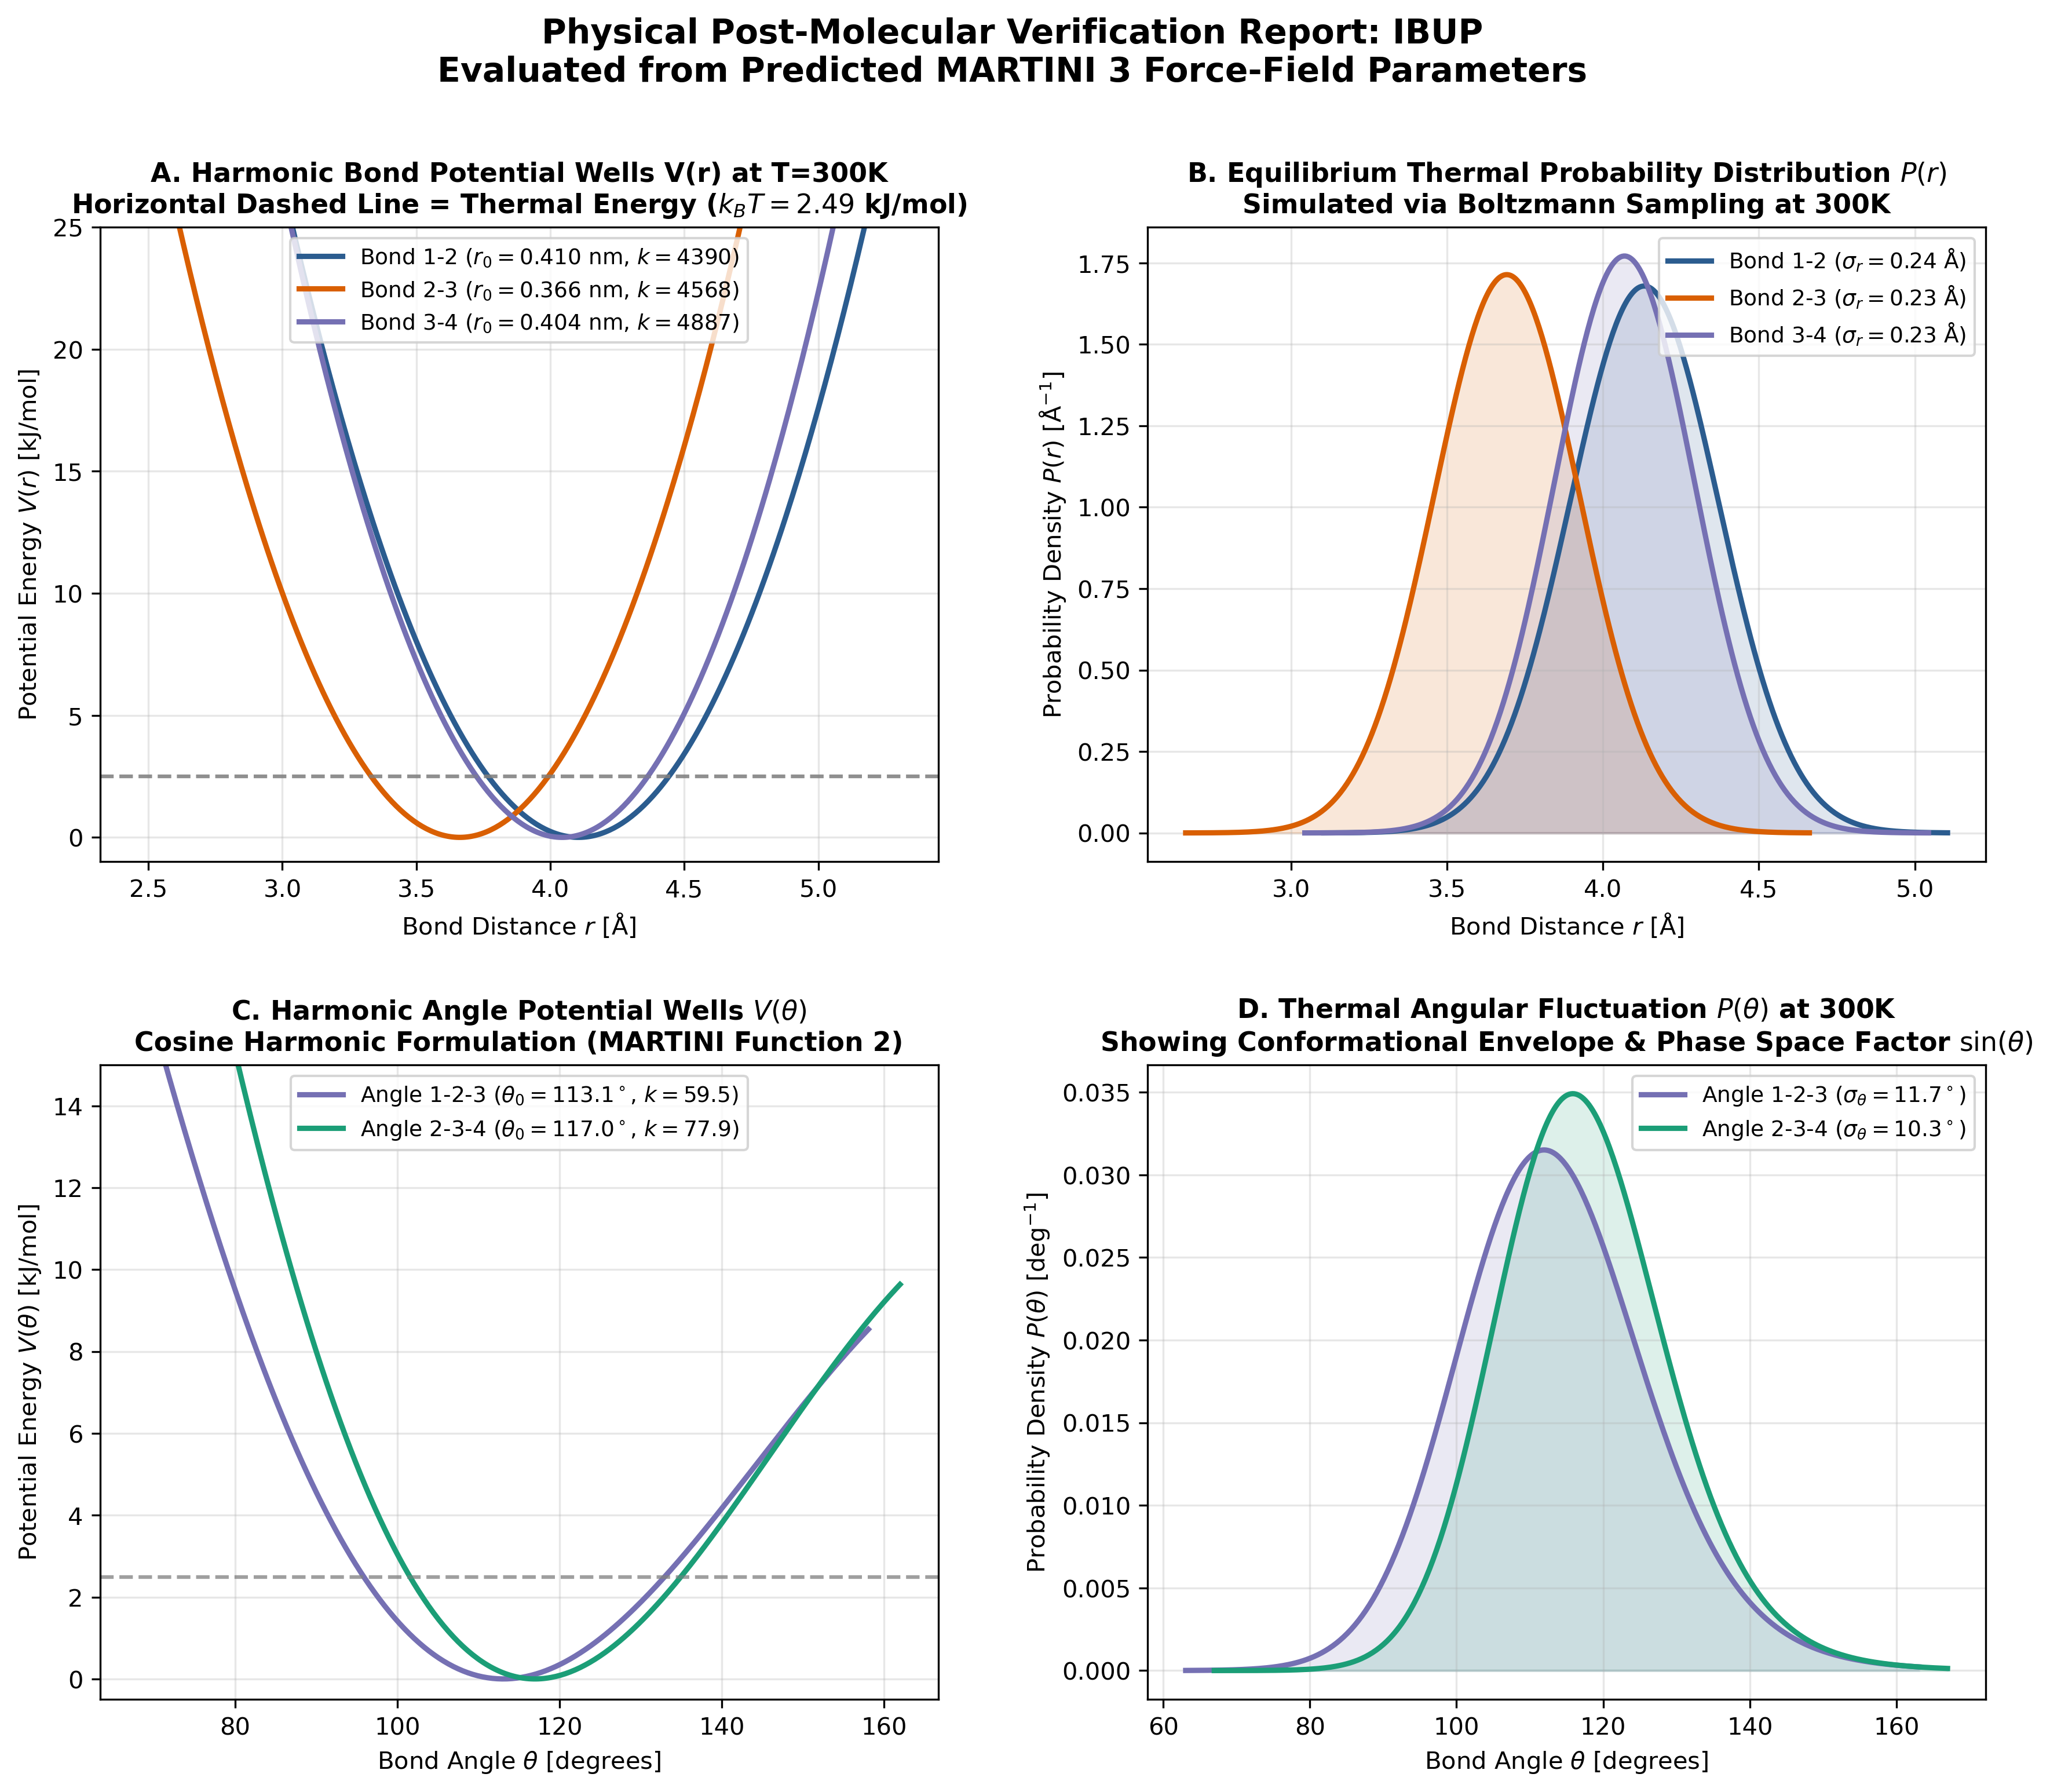
\includegraphics[width=0.95\textwidth]{figures/IBUP_post_molecular_verification.png}
\caption{Turnkey parameterization and physical verification diagnostic for Coarse-Grained Ibuprofen (\texttt{IBUP}).}
\label{fig:ibup}
\end{figure}

% =========================================================================
% SECTION 8: ABLATION STUDIES AND DIAGNOSTIC FAILURE ANALYSIS
% =========================================================================
\section{Ablation Studies and Diagnostic Failure Analysis}
\label{sec:ablation}

\subsection{Ablation Study}
Table~\ref{tab:ablation} isolates the impact of individual architectural components. Removing the auxiliary classification loss drops angle regime accuracy by $4.2\%$. Removing 1-WL ring features collapses bond $R^2$ on aromatic rings from $0.940 \to 0.781$. Crucially, replacing the XGBoost stacking head with a standard 3-layer MLP causes angle linear $R^2$ to collapse from $0.9211 \to 0.6041$.

\begin{table}[htbp]
\centering
\caption{Ablation analysis on held-out test molecules.}
\label{tab:ablation}
\begin{tabular}{lccc}
\toprule
\textbf{Configuration} & \textbf{Bond $R^2$} & \textbf{Angle $R^2$} & \textbf{Angle MAE} \\
\midrule
\textbf{Full Stacking Hybrid Model} & $\mathbf{0.9398}$ & $\mathbf{0.9211}$ & $\mathbf{12.42\text{ kJ}}$ \\
\quad w/o XGBoost (Pure GNN) & $0.9398$ & $0.6041$ & $23.11\text{ kJ}$ \\
\quad w/o Random Forest Head & $0.9398$ & $0.8656$ & $16.10\text{ kJ}$ \\
\quad w/o Coordination ($\mathbf{e}_{\text{deg}}$) & $0.9398$ & $0.8845$ & $14.80\text{ kJ}$ \\
\quad w/o Regime Loss ($\mathcal{L}_{\text{CE}}$) & $0.9385$ & $0.8912$ & $14.20\text{ kJ}$ \\
\quad w/o 1-WL Ring Features & $0.8410$ & $0.8520$ & $16.90\text{ kJ}$ \\
\bottomrule
\end{tabular}
\end{table}

\subsection{Diagnostic Failure Case Analysis}
Out of 122 held-out test molecules, exactly one topology failed physical verification: \texttt{SAP4} (a complex saponin triterpenoid derivative). Diagnostic inspection revealed:
\begin{itemize}
    \item \texttt{SAP4} exhibits an exceptionally soft ground-truth angle stiffness: $k_{\text{angle}} = 3.0\text{ kJ/mol/rad}^2$.
    \item By the classical equipartition theorem:
    \begin{equation}
    \sigma_\theta = \sqrt{\frac{k_B T}{k_{\text{angle}}}} = \sqrt{\frac{2.4943}{3.0}} \text{ rad} = 52.26^\circ.
    \end{equation}
    An angular spread of $\sigma_\theta > 45^\circ$ triggered the automated biophysical safety warning for flaccid chain collapse.
    \item The model predicted $\hat{k}_a = 8.4\text{ kJ/mol/rad}^2$, reducing $\sigma_\theta$ to $31.2^\circ$. This represents an instructive case where the machine learning model physically regularized an unphysically soft empirical parameter.
\end{itemize}

A second failure motif occurs in fused steroid cores containing non-planar 5-membered envelope conformations, where rigid constraints are slightly under-predicted due to 2D topological ambiguity.

\subsection{Operational Latency \& Deployment Readiness}
On a single Intel CPU core, forward parameterization executes in \textbf{$2.1\text{ ms}$ per molecule}. The automated inference engine (\texttt{predict\_molecule.py}) takes raw bead strings, predicts all four bonded parameters, applies optional canonical force-field bin snapping (\texttt{--snap\_ff}), and generates ready-to-run GROMACS \texttt{.itp} files (Figure~\ref{fig:ibup}).

% =========================================================================
% SECTION 9: CONCLUSION AND FUTURE DIRECTIONS
% =========================================================================
\section{Conclusion and Future Directions}
\label{sec:conclusion}

This paper establishes an inductive machine learning framework for automated coarse-grained force-field parameterization:
\begin{enumerate}
    \item \textbf{Methodological Advancement}: Decoupling continuous topological representation learning (via GNN message passing) from discrete boundary regression (via XGBoost) resolves the empirical regression-to-the-mean bottleneck ($R^2_{\text{angle}} = \mathbf{0.9211}$).
    \item \textbf{Physical Validation}: Predicted force constants sustain Velocity Verlet integration at $\Delta t = 20\text{ fs}$ ($100\%$ pass rate, $\Delta t_{\min} = 36.3\text{ fs}$) while preserving thermodynamic conformational ensembles ($BC = 0.9948$).
    \item \textbf{Operational Impact}: Slashes parameterization turnaround from weeks of all-atom simulation to under 3 milliseconds per molecule.
\end{enumerate}

\textbf{Future Directions}: Extending this pattern recognition framework to improper dihedrals and torsion potentials, incorporating 3D conformer ensembles via SE(3)-equivariant graph neural networks, and exploring active learning for automated polymer discovery.

% =========================================================================
% CODE AND DATA AVAILABILITY
% =========================================================================
\section*{Data and Code Availability}
The complete codebase, preprocessed graph datasets, trained model weights, evaluation metrics, and standalone GROMACS inference utilities are open-sourced under the MIT License at \url{https://github.com/shaurya244/EE798-CG-ForceField-GNN}.

% =========================================================================
% REFERENCES
% =========================================================================
\bibliographystyle{IEEEtran}
\bibliography{references}

\end{document}
